\definecolor{exxetagray}{gray}{0.75}
\definecolor{itemcolor}{RGB}{179,217,255}
\definecolor{usercolor}{RGB}{255,204,179}

\shorthandoff{"}
\chapter{Empfehlungssysteme}
\label{ch:empfehlungssysteme}

\section{Einführung}
\label{ch:empfehlungssysteme:einführung}
Grundsätzlich können Empfehlungssysteme (engl.: \acp{RS}) als Techniken und Werkzeuge \cite[S. 4]{ricci:inbook}\cite[S. 1]{yadav:inproceedings} verstanden werden, die einem Nutzer oder einer Gruppe von Nutzern eines Systems, aus einer Menge möglicher Entitäten, potenziell nützliche Elemente vorschlagen.
% Nach \textcite[S. 4]{ricci:inbook} können Empfehlungssysteme (engl.: \ac{RS}) allgemein als Techniken und Werkzeuge verstanden werden, die einem Nutzer oder einer Gruppe an Nutzern eines Systems, aus einer Menge möglicher Entitäten, potenziell nützliche Elemente vorschlagen.
% Allgemein können Empfehlungssysteme (engl.: \ac{RS}) als Techniken und Werkzeuge verstanden werden, die einem Nutzer oder einer Gruppe an Nutzern eines Systems, aus einer Menge möglicher Entitäten, potenziell nützliche Elemente vorschlagen \cite[S. 4]{ricci:inbook}\cite[S. 1]{klahold:book}.
% Im einfachsten Sinne können Empfehlungssysteme (engl.: \ac{RS}) als Techniken und Werkzeuge verstanden werden, die Nutzern eines Systems aus einer Menge an Elementen potenziell nützliche Elemente vorschlagen \cite[S. 10]{ricci:inbook}.
% Etwas feingranularer definiert \textcite[S. 1]{klahold:book} Empfehlungssysteme als Systeme, die einem Nutzer oder einer Gruppe an Nutzern in einem gegebenen Kontext aus einer Menge möglicher Entitäten eine Teilmenge "nützlicher" Elemente empfehlen.
% Aus der Definition von \textcite[S. 4]{ricci:inbook} lassen sich grundlegende Komponenten, die für das Erstellen von Empfehlungen in Empfehlungssystemen von Bedeutung sind, abgrenzen.
Aus diesem Verständnis lassen sich grundlegende Komponenten, die für das Erstellen von Empfehlungen in Empfehlungssystemen von Bedeutung sind, ableiten.
Deren Zusammenspiel ist in Abbildung \ref{fig:empfehlungssysteme:einführung:abb1} dargestellt.
% Für ein fundiertes Verständnis sind die einzelnen Komponenten und deren Zusammenspiel in Abbildung \ref{fig:empfehlungssysteme:einführung:abb1} dargestellt.

\begin{figure}[H]
    \centering
	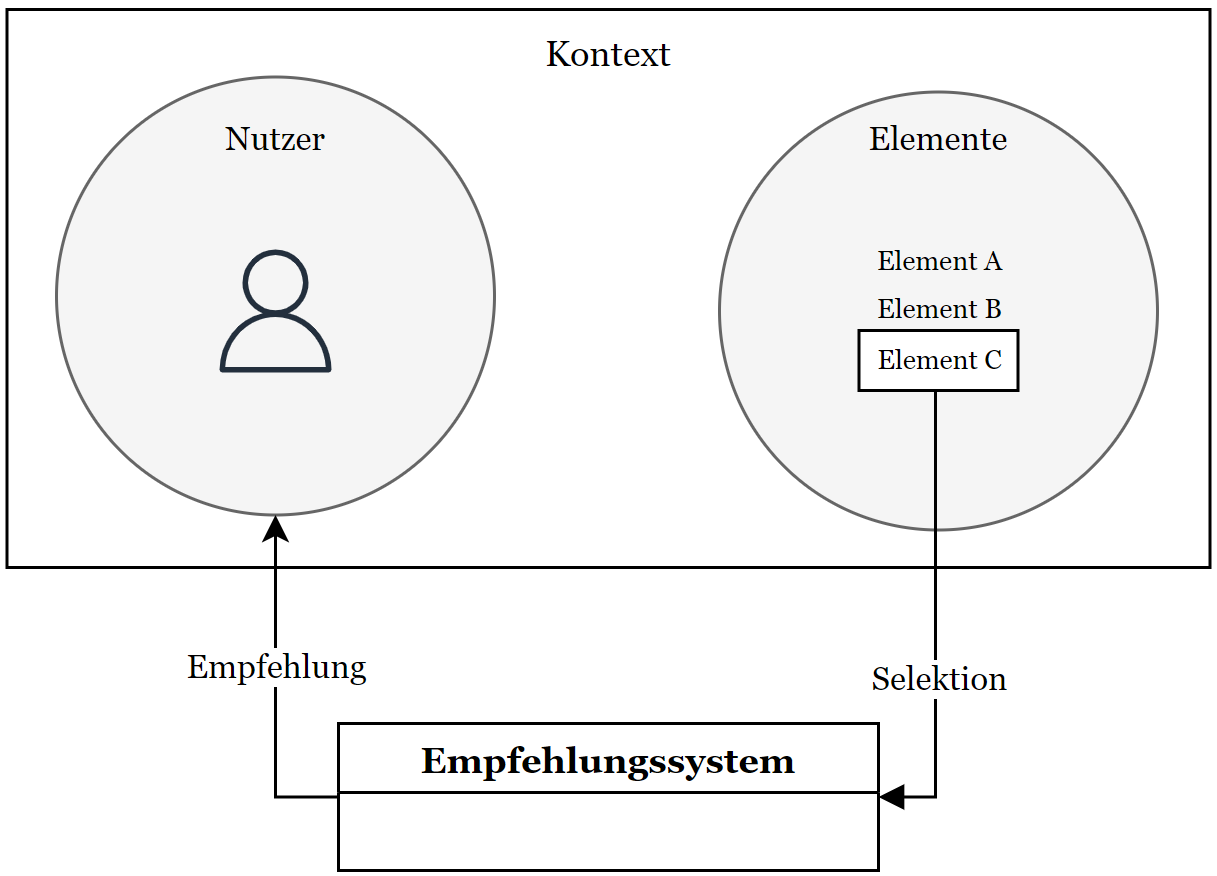
\includegraphics[width=0.8\textwidth]{gfx/komponenten-empfehlungssystem.png}
	\caption[Übersicht Empfehlungssystem]{Übersicht Empfehlungssystem\\
	(Eigene Darstellung in Anlehnung an \cite[S. 2]{klahold:book})}
	\label{fig:empfehlungssysteme:einführung:abb1}
\end{figure}

Wie aus Abbildung \ref{fig:empfehlungssysteme:einführung:abb1} hervorgeht, stehen sich bei Empfehlungssystemen grundsätzlich zwei Komponenten gegenüber.
Auf der einen Seite stehen Empfänger von Vorschlägen, welche in Empfehlungssystemen als Nutzer bezeichnet werden \cite[S. 8]{ricci:inbook}.
Auf der anderen Seite stehen Entitäten, die den Anwendern eines Systems empfohlen werden können.
Entitäten werden in Empfehlungssystemen als Elemente bezeichnet und bilden den Inhalt von Empfehlungen.
Dabei kann es sich bei Elementen sowohl um Gegenstände wie CDs, Bücher und Hotels handeln, als auch beispielsweise um Personen, Orte oder Prozesse \cite[S. 4]{klahold:book}.
% Unter dem Kontext einer Empfehlung versteht \textcite[S. 1]{klahold:book} das Zusammenspiel aus der Situation, in der eine Empfehlung gegeben wird, dem Profil eines Nutzers sowie der Menge möglicher Entitäten zum Zeitpunkt einer Empfehlung.
% Unter dem Kontext einer Empfehlung verstehen \textcite[S. 191]{adomavicius:3:inbook} zusätzliche Parameter wie Uhrzeit, Ort oder die Gegenwart anderer Personen zum Zeitpunkt einer Empfehlung.\footnote{\textcite[S. 1]{klahold:book} versteht unter dem Kontext das Zusammenspiel aus der Situation, in der eine Empfehlung gegeben wird, dem Profil eines Nutzers sowie der Menge möglicher Entitäten zum Zeitpunkt einer Empfehlung. Es wird angenommen, dass der Kontext nach dem Verständnis von \textcite{ricci:book} gleichzusetzen ist mit der Situation nach dem Verstängnis von \textcite{klahold:book} und die Berücksichtigung von Nutzerprofil und Elementen nach dem Verständnis von \textcite{ricci:book} implizit stattfindet.}

Nutzer und Elemente können in Empfehlungssystemen miteinander in Beziehung stehen.
Grundlage dieser Beziehungen bilden dokumentierte Interaktionen zwischen Nutzern und Empfehlungssystem, wie der Kauf oder die Bewertung eines Produktes durch einen Anwender.
Dokumentierte Interaktionen werden in Empfehlungssystemen als Transaktion bezeichnet \cite[S. 9]{ricci:inbook}.

Die bekannteste Form der Transaktion stellen Bewertungen dar \cite[S. 9]{ricci:inbook}.
Bewertungen von Elementen in Empfehlungssystemen können sowohl explizit als auch implizit erfolgen.
Unter expliziter Bewertung wird in Empfehlungssystemen die ausdrückliche Bewertung eines Elements durch einen Nutzer verstanden \cite[S. 9]{ricci:inbook}.
Ein Beispiel stellt die aktive Bewertung eines Produktes durch einen Nutzer in einem Online-Shop in Form einer Produktrezension (z.B. "Gefällt-mir"-Angabe) dar.
Im Vergleich dazu werden unter impliziten Bewertungen passiv erzeugte Verhaltensdaten wie der Suchverlauf oder die Kaufhistorie eines Nutzers verstanden, die indirekt mögliche Präferenzen eines Nutzers vermuten lassen \cite[S. 149]{jadidinejad:inproceedings}\cite[S. 403]{unternährer:article}.
% \textcite[S. 8]{recommenderSystems:2016} bezeichnet Bewertungen in Empfehlungssystemen auch als Nutzer-Element-Interaktionen.

Neben Transaktionen können Nutzer bzw. Elemente in Empfehlungssystemen zusätzlich Attribute besitzen \cite[S. 735]{adomavicius:inproceedings}\cite[S. 8]{recommenderSystems:2016}.
Beispiele für Attribute eines Nutzers sind Geschlecht oder Alter eines Anwenders, während Attribute eines Elements beispielsweise Produktkategorie oder beschreibende Schlagwörter darstellen.
% Unterschied Kombination und Interaktion? Kombination ist nicht zwangsläufig das vorhandensein einer Interaktion

\section{Problemstellung}
\label{ch:empfehlungssysteme:problemstellung}
% Im vorangegangenen Kapitel wurden grundlegende Komponenten von Empfehlungssystemen und deren Zusammenspiel erläutert.
% Das grundlegende Problem in Empfehlungssystemen besteht in der Auswahl der Elemente aus einer Menge an Entitäten, von denen angenommen werden kann, dass diese für die Empfänger einer Empfehlung von Relevanz sind \cite[S. 734f.]{adomavicius:inproceedings}\cite[S. 76]{jannach:inproceedings}.
% Das grundlegende Problem in Empfehlungssystemen besteht in der Auswahl der Elemente, von denen angenommen werden kann, dass diese für die Empfänger einer Empfehlung von Relevanz sind \cite[S. 734f.]{adomavicius:inproceedings}\cite[S. 76]{jannach:inproceedings}.
% Relevanz bedeutet in dem Kontext von Empfehlungssystemen, dass ein Element für einen Nutzer bzw. eine Gruppe an Nutzern einen maximalen Nutzen bietet \cite[S. 49f.]{adomavicius:inproceedings:2}\cite[S. 219]{lakiotaki:inproceedings}.
% Formal ausgedrückt besteht das Problem darin, einem Nutzer $c \in C$ eine Menge an Elementen $s^{'}$ $\in$ $S$ zur Verfügung zu stellen, für die gilt:
\textcite[S. 735]{adomavicius:inproceedings} formulieren die grundlegende Problemstellung in Empfehlungssystemen wie folgt:
\begin{equation}\label{eq1}
    \forall c \in C, s'_c = arg\max_{s \in S} u(c,s)
\end{equation}
Hierbei bezeichnet $C$ die Menge aller Nutzer und $S$ die Menge aller Elemente eines Systems.
Nach \textcite[S. 735]{adomavicius:inproceedings} gibt $u(c,s)$ den Nutzen eines Elements $s$ für einen Nutzer $c$ an und $s'_c$ das Element mit maximalem Nutzen für den Nutzer $c$, welches diesem empfohlen wird.

Bei dem beschriebenen Problem in Gleichung \ref{eq1} handelt es sich um ein Maximierungsproblem.
Nach \textcite[S. 1]{book:kallrath} können Maximierungsprobleme der Kategorie der Optimierungsprobleme zugeordnet werden.
Die Problematik des Ermittelns einer nutzenmaximierenden Teilmenge aus einer Menge von Elementen gehört demnach zu der Kategorie der Optimierungsprobleme.
% Da es sich bei dem Problem des Ermittelns einer nutzenmaximierenden Teilmenge aus einer Menge an Elementen um ein Maximierungsproblem handelt, kann das Problem der Kategorie der Optimierungsprobleme, wie in \textcite[S. 1]{book:kallrath} definiert, zugeordnet werden.

In der Literatur ist der Nutzen $u(c,s)$ einer Kombination $(c,s)$ an Nutzer $c$ und Element $s$ (im Folgenden \ac{N-E-K} genannt \cite[S. 3]{recommenderSystems:2016}) nicht eindeutig definiert.
% Wird das Problem aus Gleichung \ref{eq1} auf einem höheren Abstraktionslevel betrachtet, besteht das grundsätzliche Problem in Empfehlungssystemen in der Auswahl von Elementen $s' \in S$ für einen Nutzer $c \in C$ mit maximalem Nutzen $u(c,s)$.
Nach \textcite[S. 1]{jannach:article} betrachtet ein Großteil der Forschungsarbeiten Empfehlungssysteme aus Sicht der Empfehlungsempfänger.
Das allgemeine Problem in solchen Systemen besteht darin, den Nutzen für einen Anwender zu maximieren, indem Elemente empfohlen werden, die für den Anwender potenziell von Relevanz sind \cite[S. 1]{jannach:article}.
Unter dem Nutzen einer \ac{N-E-K} wird in der Literatur folglich überwiegend der Wert eines Elements für einen Nutzer verstanden \cite[S. 735]{adomavicius:inproceedings}\cite[S. 1]{klahold:book}\cite[S. 3880]{nilashi:article}\cite[S. 10f.]{ricci:inbook}.

Empfehlungssysteme können auch aus Sicht des Dienstleisters (z.B. Online-Händler \cite[S. 347]{abdollahpouri:inproceedings}\cite[S. 1]{jannach:article}\cite[S. 231]{sahoo:article}) eines Systems betrachtet werden \cite[S. 2]{jannach:2:inproceedings}.
Von dem Standpunkt eines Dienstleisters aus bewirkt eine Empfehlung der relevantesten Elemente für einen Nutzer nicht zwangsläufig einen maximalen Nutzen \cite[S. 1]{jannach:article}.
Sind beispielsweise zwei Produkte in einem Online-Shop interessant für einen Kunden, so kann es aus Sicht des Shop-Betreibers nützlicher sein, dem Kunden das Produkt zu empfehlen, das zu einem höheren Gewinn für den Shop-Betreiber führt.
Aus dieser Perspektive kann Nutzen in Empfehlungssystemen demnach auch als Wert einer \ac{N-E-K} für den Dienstleister verstanden werden.

Wird die Problemstellung aus Gleichung \ref{eq1} daher weiter verallgemeinert, kann das grundlegende Problem in Empfehlungssystemen als Auswahl der Elemente $s'$$\in$$S$ für einen Nutzer $c$$\in$$C$ mit maximalem Nutzen $u(c,s)$ verstanden werden.
% Das Problem in Gleichung \ref{eq1} kann abstrahiert werden als das grundsätzliche Problem der Auswahl von Elementen $s' \in S$ für einen Nutzer $c \in C$ mit maximalem Nutzen $u(c,s)$. % verallgemeinert werden?
Dabei bleibt vorerst offen, was im Einzelfall unter dem Nutzen $u(c,s)$ einer \ac{N-E-K} verstanden wird.
Diese Verallgemeinerung ermöglicht eine Formulierung des Problems, die für alle Empfehlungssysteme zutreffend ist.

% Der Kontext $K$ wird in \textcite[S. 1]{klahold:book} explizit für die Ermittlung des Nutzen einer Nutzer- Element- Kombination angeführt.
% Unter dem Kontext einer Empfehlung verstehen \textcite[S. 191]{adomavicius:3:inbook} zusätzliche Parameter wie Uhrzeit, Ort oder die Gegenwart anderer Personen zum Zeitpunkt einer Empfehlung.
% Grundsätzlich stellen kontextbasierte Empfehlungssysteme, das heißt Syteme, die den Kontext von Empfehlungen für die Ermittlung des Nutzen berücksichtigen, eine Erweiterung traditioneller Empfehlungssyteme dar \cite[S. 744ff.]{adomavicius:inproceedings}.
% In der Literatur wird der Nutzen einer Nutzer- Element- Kombination traditionell ohne Berücksichtigung des Kontextes betrachtet, weshalb der Kontext von Empfehlungen in dieser Arbeit vernachlässigt wird \cite[S. 734f.]{adomavicius:inproceedings}\cite[S. 219]{lakiotaki:inproceedings}\cite[S. 3]{jawaheer:article}.
% In Anlehnung an \textcite[S. 3]{jawaheer:article} wird der interessierte Leser für eine detaillierte Übersicht zu kontextbasierten Empfehlungssystemen auf \textcite[S. 191ff]{adomavicius:3:inbook} verwiesen.
% In den Formulierungen der Gleichung in \cite[S. 734f]{adomavicius:inproceedings} und \cite[S. 219]{lakiotaki:inproceedings} wird jedoch nicht explizit auf den Kontext als Bedingung zur Erfüllung von Gleichung \ref{eq1} hingewiesen.
% Es wird angenommen, dass der Kontext für die Ermittlung der Güte einer Empfehlung implizit berücksichtigt wird und daher auf eine explizite Nennung verzichtet wurde. In Anlehnung an \cite[S. 734f]{adomavicius:inproceedings} und \cite[S. 219]{lakiotaki:inproceedings} wurde daher auf die explizite Unterscheidung im weiteren Verlauf verzichtet.

% Einigung: Nützlichkeit bezieht sich nicht auf die Güte einer Empfehlung, sondern auf den Nutzen einer Kombination. Güte beschreibt Wert einer Empfehlung.
% Der Begriff der "Nützlichkeit" wird in der Literatur überwiegend verwendet, um den Wert eines Elements für einen Nutzer zu beschreiben \cite[S. 10f.]{ricci:inbook}\cite[S. 1]{klahold:book}\cite[S. 735]{adomavicius:inproceedings}.\footnote{Unter der Nützlichkeit kann in dem Kontext von Empfehlungssystemen auch die Güte einer Empfehlung verstanden werden \cite[S. 37ff.]{klahold:book}.}
Der Nutzen kann sowohl unmittelbar über Angaben eines Nutzers erschlossen, als auch über eine Nutzenfunktion des Empfehlungssystems berechnet werden \cite[S. 735]{adomavicius:inproceedings}.
Da die Ermittlung des Nutzens durchaus komplex sein kann, wird die Nutzenfunktion anschließendend in Kapitel \ref{ch:empfehlungssysteme:nutzenfunktion} ausführlich erläutert.

\section{Nutzenfunktion}
\label{ch:empfehlungssysteme:nutzenfunktion}
% Frage: ist mit der Güte die Güte einer Empfehlung gemeint (gefällt einem nutzer die Empfehlung ja/nein), oder ist damit die Güte im Sinne von die Qualität von Empfehlungssystemen gemeint?
% Der erfolgreiche Einsatz von Empfehlungssystemen wird maßgeblich von der Qualität der ausgesprochenen Empfehlungen bestimmt.
Wie aus Gleichung \ref{eq1} hervorgeht, wird für den Nutzen einer \ac{N-E-K} in Empfehlungssystemen allgemein eine Funktion $u$ angenommen.
Diese Funktion wird Nutzenfunktion (engl.: utility function) genannt und ist traditionell definiert als \cite[S. 195]{adomavicius:3:inbook}\cite[S. 1156]{gupta:inproceedings}\cite[S. 3]{jawaheer:article}\cite[S. 219]{lakiotaki:inproceedings}\cite[S. 3880]{nilashi:article}:
\begin{equation}\label{eq2}% Dabei handelt es sich um eine lineare Abbildung, bei der über die Funktion u jeder Kombination aus der nxm matrix, genau ein Wert aus R, also der Rating matrix, zugeordnet werden kann
    u: Nutzer \times Element \rightarrow R_{0}
\end{equation}
Über die Nutzenfunktion $u(c_{i},s_{j})$ kann jeder Kombination $(c_{i},s_{j})$ von Nutzer $c_{i}$ und Element $s_{j}$ eines Empfehlungssystems ein Nutzen $u_{c_{i},s_{j}} \in R_{0}$ zugeordnet werden.
$R_{0}$ stellt in der Regel eine geordnete Menge dar, die alle Werte umfasst, die der Nutzen einer Kombination annehmen kann (z.B. $R_{0} = [1,5]$) \cite[S. 49]{adomavicius:inproceedings:2}.

Die Nutzenfunktion $u$ kann auch als Matrix $u[.,.]$ abgebildet werden \cite[S. 1]{dekhtyar:misc}.
Jeder Eintrag $u_{c_{i}s_{j}}$ der Matrix stellt den Nutzen $u(c_{i},s_{j})$ einer \ac{N-E-K} aus Element $s_{j}$ und Nutzer $c_{i}$ dar (d.h. $u(c_{i},s_{j}) = u_{c_{i}s_{j}}$) \cite[S. 1]{dekhtyar:misc}.
% In Systemen, in denen der Wert einer Transaktion beispielsweise über eine explizite, binäre Bewertung (z.B. "Gut", "Schlecht") eines Nutzers für ein Element bestimmt wird, würde $R_{0}$ genau die zwei Ausprägungen umfassen, die eine Bewertung annehmen kann (hier: "Gut" und "Schlecht").

Grundsätzlich kann die Nutzenfunktion in Empfehlungssystemen jede beliebige Funktion darstellen \cite[S. 735]{adomavicius:inproceedings}.
Besteht das Ziel eines Empfehlungssystems bespielsweise darin, den Gesamtumsatz eines Unternehmens zu maximieren, so kann der Nutzen einer \ac{N-E-K} über eine Profit-Funktion ermittelt werden \cite[S. 735]{adomavicius:inproceedings}\cite[S. 896]{adomavicius:article}\cite[S. 11]{recommenderSystems:2016}\cite[S. 1]{jannach:article}.
% $R(c,s)$ würde dann den Nutzen einer Kombination von Nutzer und Element aus Sicht des Unternehmens, welches den Empfehlungsservice einsetzt, darstellen \cite[S. 1]{jannach:article}.
% Solche Systeme, in denen der Nutzen von Nutzer- Element- Kombinationen über eine eigenständige Nutzenfunktion ermittelt wird, zählen zu den nutzenbasierten Empfehlungssystemen und sind nicht Inhalt dieser Arbeit.
In den meisten Empfehlungssystemen wird für den Nutzen $u(c,s)$ einer Kombination unmittelbar die Bewertung (engl.: Rating) eines Element $s$ durch einen Nutzer $c$ angenommen \cite[S. 735]{adomavicius:inproceedings}\cite[S. 1]{dekhtyar:misc}\cite[S. 3880]{nilashi:article}\cite[S. 11]{recommenderSystems:2016}\cite[S. 9]{ricci:inbook}.
Bewertungen von Nutzern für Elemente werden in Empfehlungssystemen grundsätzlich in einer $Nutzer \times Element$-Matrix abgebildet, welche als Rating-Matrix $R$ bezeichnet wird \cite[S. 87]{ekstrand:article}.
Nach \textcite[S. 48f.]{adomavicius:inproceedings:2} können Bewertungen in Empfehlungssystemen über eine Ratingfunktion $R(c,s)$ bestimmt werden, welche wie folgt definiert ist:
\begin{equation}\label{eq10}
    R: Nutzer \times Element \rightarrow Rating
\end{equation}
Über die Ratingfunktion $R(c_{i},s_{j})$ kann jeder \ac{N-E-K} $(c_{i},s_{j})$ von Nutzer $c_{i}$ und Element $s_{j}$ eine Bewertung $r_{c_{i},s_{j}} \in Rating$ zugeordnet werden \cite[S. 42]{ning:inbook}.
$Rating$ stellt eine Sammlung aller Werte dar, die eine Bewertung annehmen kann (z.B. $Rating = [1,5]$) \cite[S. 41]{ning:inbook}.

Da Nutzen und Rating in der Literatur häufig synonym verwendet werden \cite[S. 11]{recommenderSystems:2016}, wird die Nutzenfunktion auch als Ratingfunktion \cite[S. 49]{adomavicius:inproceedings:2} oder Rating-Matrix \cite[S. 87]{ekstrand:article} bezeichnet.
Aus Gründen der Einfachheit wird für den weiteren Verlauf der Arbeit ebenfalls der Wert einer Bewertung $r_{cs}$ für den Nutzen $u_{cs}$ einer \ac{N-E-K} $(c,s)$ angenommen (d.h. $r_{cs} = u_{cs}$).
Wenn nicht ausdrücklich angeführt, werden die Begrifflichkeiten Nutzenfunktion, Ratingfunktion und Rating-Matrix daher nachfolgend synonym verwendet.

% Diese Abbildung einer Funktion als Matrix folgt der mathematischen Definition von Matrizen als lineare Funktion.
% Es wird davon ausgegangen, dass die gängige Verwendung des Ratings als Maß des Nutzen eines Elements für einen Nutzer daher kommt, dass Empfehlungssysteme traditionell in dem Kontext item-to-people-recommendation eingesetzt wurden.
% In solchen systemen ist es meistens das ziel, die elemente zu empfehlen, die den nutzer am meisten ansprechen. -> Folglich Nutzen einer Nutzer-Element-Kombination bedeutet Nutzen eines Elements für einen Nutzer. (kann aber ja auch bedeuten nutzen eines elements für einen nutzer im sinne von profitmaximierung)
% Unter der Annahme ist damit erklärbar, dass mit einer gewissen Konfidenz davon ausgegangen werden kann, dass die Bewertung eines Nutzers für ein Element auch dessen gefühlten Nutzen des ELements für ihn abbildet.

%Bewertungen von Elementen in Empfehlungssystemen können sowohl explizit als auch implizit erfolgen.
%Unter expliziter Bewertung kann in Empfehlungssystemen die ausdrückliche Bewertung eines Elements durch einen Nutzer verstanden werden.
%Ein Beispiel stellt die aktive Bewertung eines Produktes durch einen Nutzer in einem Online-Shop in Form einer Produktrezension (z.B. "Gefällt-mir"-Angabe) dar.
%Im Vergleich dazu werden unter impliziten Bewertungen in Empfehlungssystemen passiv erzeugte Verhaltensdaten, wie der Suchverlauf oder die Kaufhistorie eines Nutzers, verstanden, die indirekt mögliche Präferenzen eines Nutzers vermuten lassen \cite[S. 149]{jadidinejad:inproceedings}\cite[S. 403]{unternährer:article}.
% IDEE: hier einfügen Rating Scales? Ordinal, numeric, etc.

Tabelle \ref{tab1} stellt beispielhaft den Ausschnitt einer Rating-Matrix $R$ dar, welche explizite Bewertungen von Mitarbeitern zu ihren Fähigkeiten abbildet \cite[S. 735]{adomavicius:inproceedings}\cite[S. 16]{link:booklet}.
Hierbei stellen Mitarbeiter die Nutzer und Fähigkeiten die Elemente des Systems dar.
Der Wert einer \ac{N-E-K} in der Rating-Matrix gibt die Bewertung $r_{cs}$ einer Fähigkeit $s$ durch einen Mitarbeiter $c$ an.
% Der Nutzen $R(c,s)$ entspricht genau der Bewertung eines Mitarbeiters $c$ für eine Fähigkeit $s$.
Eine Bewertung kann jeden Wert in $R_{0}=\{1;2;3;4;5\}$ annehmen.

\begin{table}[htbp]
    \begin{center}
    \begin{tabular}{|c||c|c|c|c|c|c|}
    \hline
    {} & {\textbf{Java}} & {\textbf{Python}} & {\textbf{MySQL}} & {\textbf{MongoDB}} & {\textbf{HDFS}} & {\textbf{Spark}}\\
    \hline
    \hline
    \textbf{Jane D.} & ? & 4 & 3 & 3 & ? & ?\\
    \hline
    \textbf{John D.} & 3 & ? & 2 & ? & 1 & ?\\
    \hline
    \textbf{Erika M.} & ? & ? & ? & 3 & 5 & 3\\
    \hline
    \textbf{Max M.} & 2 & 3 & 1 & ? & ? & ?\\
    \hline
    \end{tabular}
    \end{center}
    \caption[Beispielhafte Darstellung einer Rating-Matrix ]{Beispielhafte Darstellung einer Rating-Matrix \\
	(Eigene Darstellung in Anlehnung an \cite[S. 16]{link:booklet})}
	\label{tab1}
\end{table}

Der Rating-Matrix $R$ können alle vorliegenden Bewertungen von Mitarbeitern zu ihren Fähigkeiten entnommen werden.
So wird beispielsweise ersichtlich, dass Jane D. im Verhältnis zu den anderen Mitarbeitern ihre Fähigkeiten in Python am höchsten bewertet hat.
Darüber hinaus geht aus Tabelle \ref{tab1} hervor, dass einige Einträge der Rating-Matrix anstelle einer Bewertung ein Fragezeichen beinhalten (z.B. $r_{Jane D.\textnormal{, Java}}=\textnormal{?}$).
Dieses kennzeichnet die \ac{N-E-K}-en des Empfehlungssystems, für die keine Bewertungen vorhanden sind.
Das kann beispielsweise bei Nutzern der Fall sein, die noch keine Elemente bewertet haben.
Auch für Elemente, die neu zu einer Anwendung hinzugefügt wurden, sind häufig noch keine Interaktionen mit Nutzern des Systems bekannt.\footnote{Das Problem ist in der Literatur als das Kaltstart-Problem bekannt \cite[S. 407]{unternährer:article}.}
Wie im nachfolgenden Kapitel deutlich werden wird, stellt die Vorhersage fehlender Transaktionenen eine der Kernaufgaben von Empfehlungssystemen dar.
% Nach \textcite[S. 37]{klahold:book} besteht eine der Herausforderungen in der Ermittlung des tatsächlichen Nutzen einer Empfehlung darin, dass für eine objektive Beurteilung die genaue Nutzenfunktion einer Empfehlung an einen Nutzer bekannt sein muss.
% Hier ergänzen nach gespräch mit Andreas. Quellen dazu: Klahod S. 37ff und hier: https://api-depositonce.tu-berlin.de/server/api/core/bitstreams/b490302e-8b6a-4300-946f-b5763c2b47d7/content

\section{Erstellen von Empfehlungen}
\label{ch:empfehlungssysteme:empfehlungserstellung}
Das Erstellen von Empfehlungen ist eine nicht-triviale Aufgabe, die bereits seit Jahrzehnten Inhalt zahlreicher Veröffentlichungen und Konferenzen ist.
Grundsätzlich kann das Erstellen von Empfehlungen in zwei Phasen unterteilt werden \cite[S. 898]{adomavicius:article}\cite[S. 854]{adomavicius:4:inbook}\cite[S. 405]{unternährer:article}:
\begin{enumerate}
	\item Vorhersage-Phase
	\item Ranking-Phase
\end{enumerate}

Üblicherweise bildet die Rating-Matrix die Ausgangslage der Empfehlungserstellung \cite[S. 48]{adomavicius:inproceedings:2}.
Basierend auf der Rating-Matrix werden in der ersten Phase des Prozesses für alle \ac{N-E-K}-en, für die keine Transaktionen vorliegen, deren Interaktion vorhergesagt \cite[S. 3]{recommenderSystems:2016}.
% Für die Ranking-Phase werden die (angenommenen) Nutzer-Element-Interakti\-onen aus Phase 1 herangezogen, in Abhängigkeit ihrer Nützlichkeit sortiert und das Element bzw. die Elemente mit dem größten Nutzen empfohlen \cite[S. 854]{adomavicius:4:inbook}.
Basierend auf den (angenommenen) Bewertungen, werden in der zweiten Phase die Elemente des Systems nach ihrer Nützlichkeit sortiert und das Element bzw. die Elemente mit dem größten Nutzen empfohlen \cite[S. 898]{adomavicius:article}.
Nachfolgend werden die einzelnen Phasen im Detail erläutert.

\subsection{Vorhersage}
\label{ch:empfehlungssysteme:empfehlungserstellung:prediction}
% Ratings normalerweise nur vorhanden bei nutzern, die diese produkte in der vergangenheit bewertet haben, S. 735, file://wsl%24/Ubuntu/home/masc6/Projects/masterarbeit/literatur/Toward_the_next_generation_of_recommender_systems_a_survey_of_the_state-of-the-art_and_possible_extensions.pdf
Wie aus Gleichung \ref{eq1} hervorgeht, ist das Vorhandensein einer Nutzer-Ele\-ment-Interaktion Voraussetzung, um die Nützlichkeit einer Kombination im Vergleich zu anderen \ac{N-E-K}-en zu bewerten.
Eine gängige Eigenschaft von Umgebungen, in denen Empfehlungssysteme ihren Einsatz finden, ist, dass die zugrundeliegenden Daten unvollständig sind \cite[S. 735]{adomavicius:inproceedings}.\footnote{Dieses Problem wird in der Literatur als Sparsity-Problem bezeichnet \cite[S. 61]{ning:inbook}.}
Das bedeutet, dass nicht für jede Kombination an Nutzer und Element ein Wert für $r_{cs}$ vorliegt (wie in Tabelle \ref{tab1} durch Fragezeichen gekennzeichnet).
So ist es beispielsweise anhand der Daten aus Tabelle \ref{tab1} nicht möglich zu Beurteilen, welche der beiden Mitarbeiter Jane D. und Erika M. die Fähigkeit Java besser beherrscht.
% Würde beispielsweise für Erika M. aus Tabelle \ref{tab1} versucht zu Bestimmen, ob ihre Fähigkeiten in Java oder Python höher sind, könnte anhand von Gleichung \ref{eq1} aufgrund der fehlenden Transaktion keine Aussage getroffen werden.

Aufgabe eines Empfehlungssystems ist es daher, die fehlenden Bewertungen für \ac{N-E-K}-en der Rating-Matrix $R$ vorherzusagen.
Sei $\hat{r}_{cs}$ der angenommene Wert einer Transaktion in einem Empfehlungssystem, so wird $\hat{r}_{cs}$ allgemein wie folgt vorhergesagt (in Anlehnung an \cite[S. 743]{adomavicius:inproceedings}):\footnote{Voraussetzung der Gültigkeit der Formel \ref{eq3} ist die Annahme, dass gilt $r_{cs} = R(c,s)$. Das bedeutet, dass für den Nutzen einer \ac{N-E-K} unmittelbar der Wert der Bewertung $r_{cs}$ eines Nutzers $c$ für das Element $s$ angenommen werden kann (Vgl. Kapitel \ref{ch:empfehlungssysteme:nutzenfunktion}).}
% Für die Vorhersage einer Nutzer- Element- Kombination $\hat{r}_{cs}$ der Matrix R kann allgemein folgende Formel angenommen werden (in Anlehnung an \cite[S. 743]{adomavicius:inproceedings}):\footnote{Voraussetzung der Gültigkeit der Formel \ref{eq3} ist die Annahme, dass gilt $r_{cs} = R(c,s)$. Das bedeutet, dass für den Nutzen einer \ac{N-E-K} unmittelbar der Wert der Bewertung $r_{cs}$ eines Nutzers $c$ für das Element $s$ angenommen werden kann (Vgl. Kapitel \ref{ch:empfehlungssysteme:nutzenfunktion}).}
\begin{equation}\label{eq3}
\hat{r}_{cs} =
    \begin{cases}
        r_{cs} & \textnormal{wenn } r_{cs} \neq \textnormal{ ?} \\
        R(c,s) & \textnormal{wenn }r_{cs} = \textnormal{ ?} \\
    \end{cases}
\end{equation}
Das heißt, grundsätzlich wird $\hat{r}_{cs}$ entweder unmittelbar über vorhandene Transaktionen $r_{cs}$, oder bei fehlenden Transaktionen für $(c,s)$ unter Anwendung der Nutzenfunktion $R$ vorhergesagt.
% Demnach wird eine Bewertung $\hat{r}_{cs}$ entweder unmittelbar über vorhandene Transaktionen $r_{cs}$, oder bei fehlenden Transaktionen für $(c,s)$ unter Anwendung der Nutzenfunktion $R$ vorhergesagt werden.
% Unterschied ist, dass hier rij sich von u unterscheidet und bei uns einfach erstmal R als ein wert angenommen wird
% Wichtig hier klar zu definieren, dass die Nützlichkeit oft so definiert ist, dass sie entweder explizit gegeben ist, oder über u berechnet wird für fehlende werte von r
% bei uns wird dann quasi u für alle werte berechnet, da wir ja nicht explizit einen wert annehmen, sondern Ro sich aus r1 und r2 usw zusammensetzt

In der Praxis existieren verschiedene Techniken, um fehlende Nutzer-Ele\-ment-Interaktionen vorherzusagen.
Empfehlungssysteme können anhand der eingesetzten Technik für die Vorhersage in verschiedene Kategorien unterteilt werden \cite[S. 8 ff.]{recommenderSystems:2016}.
Zu den bekanntesten Kategorien von Empfehlungssystemen zählen:
\begin{itemize}
	\item \textit{Systeme des Kollaborativen Filterns:} Vorhersage von $\hat{r}_{cs}$ für fehlende $r_{cs}$ eines Zielnutzers $c$ anhand vorhandener Nutzer-Ele\-ment-Interaktionen $r_{c's}$ anderer Nutzer $c' \in C \backslash \{c\}$ des Systems, die dem Zielnutzer $c$ ähnlich sind \cite[S. 737]{adomavicius:inproceedings}.
	\item \textit{Inhaltsbasierte Systeme:} Vorhersage von $\hat{r}_{cs}$ für fehlende $r_{cs}$ eines Zielnutzers $c$ anhand vorhandener Nutzer-Ele\-ment-Interaktionen $r_{cs'}$ des Zielnutzers zu Elementen $s' \in S \backslash \{s\}$, die dem Zielelement $s$ ähnlich sind \cite[S. 735]{adomavicius:inproceedings}.
	\item \textit{Wissensbasierte Systeme:} Vorhersage von $\hat{r}_{cs}$ für fehlende $r_{cs}$ eines Zielnutzers unter Anwendung von spezifischem Domänenwissen und aktiv angegebener Präferenzen durch den Zielnutzer \cite[S. 16f.]{recommenderSystems:2016}.
	\item \textit{Hybride Systeme:} Kombination verschiedener Techniken für die Vorhersage fehlender Transaktionen.
\end{itemize}

Der Fokus dieser Arbeit liegt auf der zweiten Phase des Empfehlungserstel\-lungs-Prozesses, weshalb auf eine eingehende Erläuterung der Techniken nachfolgend verzichtet wird.
Für eine detaillierte Übersicht der bekanntesten Werkzeuge wird auf \textcite[S. 8ff.]{recommenderSystems:2016} verwiesen.

\subsection{Ranking}
\label{ch:empfehlungssysteme:empfehlungserstellung:recommendation}
Die zweite Phase umfasst die eigentliche Erstellung der Empfehlungen, die an einen Nutzer zurückgegeben werden.
Ziel ist es, in Abhängigkeit der vollständigen Rating-Matrix $R$ eine Empfehlung für einen Nutzer $c$ zu generieren, die das bzw. die Elemente $s'$ mit dem größtmöglichen Nutzen enthält \cite[S. 898]{adomavicius:article}\cite[S. 87]{ekstrand:article}.
% Wichtig zu unterscheiden, dass die Empfehlungen nicht zwangsäufig die präferenzen des nutzers empfehlen müssen, da diese auch von anderen kriterien abhängen könnne, siehe quelle unten

In Abhängigkeit des Anwendungsfalls kann eine Empfehlung verschiedene Formen annehmen.
So kann eine Empfehlung beispielsweise ein einizges Element umfassen (bspw. das Element mit dem größten angenommenen Nutzen für einen Nutzer) \cite[S. 6]{ricci:inbook}.
Eine Empfehlung kann auch eine Kombination unterschiedlicher Elemente darstellen \cite[S. 7]{ricci:inbook}.
Ein Beispiel stellen Empfehlungen in Online-Shops dar, die einem Kunden zu einem ausgewählten T-Shirt eine passende Hose und Schuhe vorschlagen.
Die unterschiedlichen Kleidungsstücke (Elemente) bilden gesammelt ein vollständiges Outfit, welches einem Kunden als Ganzes empfohlen werden kann.

In den meisten Fällen geben Empfehlungssysteme eine sortierte Liste an ausgewählten Elementen zurück \cite[S. 3]{recommenderSystems:2016}\cite[S. 141]{ekstrand:article}.
Diese werden auch als Top-$K$-Elemente bezeichnet.
Der Parameter $K$ gibt die Anzahl an Elementen in der Liste an.
% Dabei wird die Nützlichkeit einer \ac{N-E-K}, wie in Kapitel \ref{ch:empfehlungssysteme:empfehlungserstellung:prediction} erläutert, zumeist anhand der Bewertung eines Elements durch einen Nutzer bestimmt.
% Für \ac{N-E-K}, für die keine Bewertungen bekannt ist, wird der Nutzen einer Kombination unter Anwendung der Nutzenfunktion $R$ in Phase 1 vorhergesagt.

Nach \textcite[S. 900]{adomavicius:article} wird der Rang eines Elements in einer sortierten Liste anhand eines Sortier-Kriteriums ermittelt.
Demnach steht ein Element $s_{x}$ grundsätzlich im Ranking vor einem Element $s_{y}$, wenn $rank(s_{x})<rank(s_{y})$, wobei $rank: S \rightarrow \mathbb{R}$ eine Funktion des Sortier-Kriteri\-ums darstellt \cite[S. 900]{adomavicius:article}.
Über die Funktion wird jedem Element $s \in S$ ein Rang zugeordnet.
In der Literatur werden Elemente für Empfehlungen grundsätzlich anhand ihres Nutzen für einen Nutzer sortiert \cite[S. 735]{adomavicius:inproceedings}\cite[S. 10f.]{ricci:inbook}.
% Der Nutzen stellt daher das Sortier-Kriterium in Empfehlungssystemen dar.
% Der Nutzen kann daher als das Sortier-Kriterium in Empfehlungssystemen verstanden werden.
Wie in Kapitel \ref{ch:empfehlungssysteme:nutzenfunktion} bereits erläutert, wird für den Nutzen in Empfehlungssystemen zumeist unmittelbar das Rating eines Nutzers für ein Element angenommen.
In den meisten Empfehlungssystemen wird demnach der Rang eines Elements über das Sortier-Kriterium Rating ermittelt \cite[S. 900]{adomavicius:article}.
Dieses Rating ist in traditionellen Empfehlungssystemen häufig über eine Gesamtbewertung eines Elements durch einen Nutzer angegeben \cite[S. 219]{lakiotaki:inproceedings}.

% Es existieren verschiedene Verfahren, um den Rang eines Elements genau zu ermitteln.
% Ein bekanntes Verfahren stellt die Standard-Ranking-Methode dar, wobei der Rang eines Elements über das Inverse der (angenommenen) Gesamtbewertung eines Nutzers $c$ für das Element $s$ wie folgt bestimmt werden kann:
% \begin{equation}
%     rank_{Standard}(i) = \hat{R}(c,s)^{-1}
% \end{equation}

% In Empfehlungssystemen gibt der Nutzen $R(c,s)$ größtenteils einen Wert für eine \ac{N-E-K} zurück (z.B. eine Gesamtbewertung eines Nutzers $c$ für ein Element $s$).
% So wurde der Nutzen einer Fähigkeit in Tabelle \ref{tab1} über die Angabe eines einzigen Zahlenwertes gekennzeichnet.
% Elemente in Empfehlungssystemen können auch anhand mehrerer Kriterien bewertet werden.
% So kann ein Kinoaufenthalt (Element) beispielsweise anhand der Kriterien Inhalt und Schauspieler bewertet werden. 

% Hier geht es also quasi um den Nutzen eines Elements im Kontext einer Liste
% was ist jetzt hier der Unterschied zu kriterien die zu R hinzukommen? multicriteria hat verschiedene hintergründe, einer ist, dass Nutzen sich aus mehreren Kriterien ergibt (zb accuracy und prediction)
In der Praxis kann es vorkommen, dass eine Empfehlung der Top-$K$-Elemente mit den höchsten (angenommenen) Bewertungen nicht zwangsläufig den größten Nutzen für einen Nutzer bietet \cite[S. 896ff.]{adomavicius:article}.
So kann eine Empfehlung mit $K$ Elementen, von denen einige Elemente für einen Nutzer eher überraschend sind, für den Nutzer von größerem Interesse sein als Elemente, von denen bekannt ist, dass diese dem Nutzer gefallen \cite[S. 43]{herlocker:article}.\footnote{Der Aspekt des Empfehlens zufällig interessanter Elemente, die ein Nutzer andernfalls nicht entdeckt hätte, wird in der Literatur als Serendipität bezeichnet \cite[S. 43]{herlocker:article}\cite[S. 3]{recommenderSystems:2016}\cite[S. 1099]{mcnee:inproceedings}.}
Der Nutzen eines Elements als Bestandteil einer sortierten Liste kann folglich von mehreren Kriterien abhängen.
In solchen Empfehlungssystemen kann der Rang eines Elements anhand mehrerer Sortier-Kriterien bestimmt werden \cite[S. 405f.]{unternährer:article}.
% Der Nutzen eines Elements als Bestandteil einer Liste (d.h. der Rang des Elements) kann sich folglich von dem Nutzen einer \ac{N-E-K} unterscheiden.
% Die Frage ist also: wird mir nur ein Element empfohlen, oder eine Liste? Wird davon asugegangen, dass ein Nutzer auf eine gesamte Liste schaut oder sich nur für das gelbe vom Ei interessiert?
% Der Nutzen einer sortierten Liste ergibt sich folglich nicht zwangsläufig unmittelbar aus dem Nutzen der einzelnen \ac{N-E-K}.
% Dies hängt auch damit zusammen, dass ein Nutzer Elemente dann nicht getrennt voneinander, sondern als gesamte Empfehlung betrachtet.
% Hier den satz nach unten schieben zu MCRS und stattdessen kurz zusammenfassen, dass das Rankin einfach beeinflusst werden kann, wenn konkurrierende Ziele verfolgt werden (eben zb Accuracy und Serendipity, dann reranking).
% Das Operationalisieren des Nutzen anhand eines einzelnen Kriteriums (z.B. Rating) ist folglich nicht immer ausreichend, um den Nutzen eines Elements für einen Nutzer zuverlässig zu bestimmen \cite[S. 847]{adomavicius:4:inbook}.
% ------- Hier (oder oben?) kurze Zusammenfassung der Begrifflichkeiten (siehe aggarwal, S. xviii, file:///C:/Users/masc6/OneDrive/Persoenliche_Unterlagen/Uni/Masterthesis/Aggarwal2016_Book_RecommenderSystems.pdf)

% Weglassen?
Abbildung \ref{fig:empfehlungssysteme:recommendation:abb1} illustriert den Prozess der Empfehlungserstellung am Beispiel eines Ausschnitts der Mitarbeiter-Fähigkeiten Matrix aus Tabelle \ref{tab1}.
Das Beispiel stellt den Empfehlungerstellungsprozess für die Mitarbeiterin Erika M. dar.
Dabei soll mithilfe des Empfehlungssystems die Fähigkeit vorschlagen werden, von der angenommen werden kann, dass Erika M. in dieser Fähigkeit die meisten Kenntnisse im Vergleich zu den anderen Fähigkeiten aufweist (e.g. $argmax(\hat{r}_{\textnormal{Erika M., s}})$).
% am die dieser am Gesucht: Element des Mitarbeiters, für das er/sie die höchsten Fähigkeiten aufweist, bspw. weil vorgeschalgen wird in dem Bereich eine Schulung zu geben, oder MA gesucht wird, der experte in einem bestimmten gebiet ist

\begin{figure}[H]
    \centering
	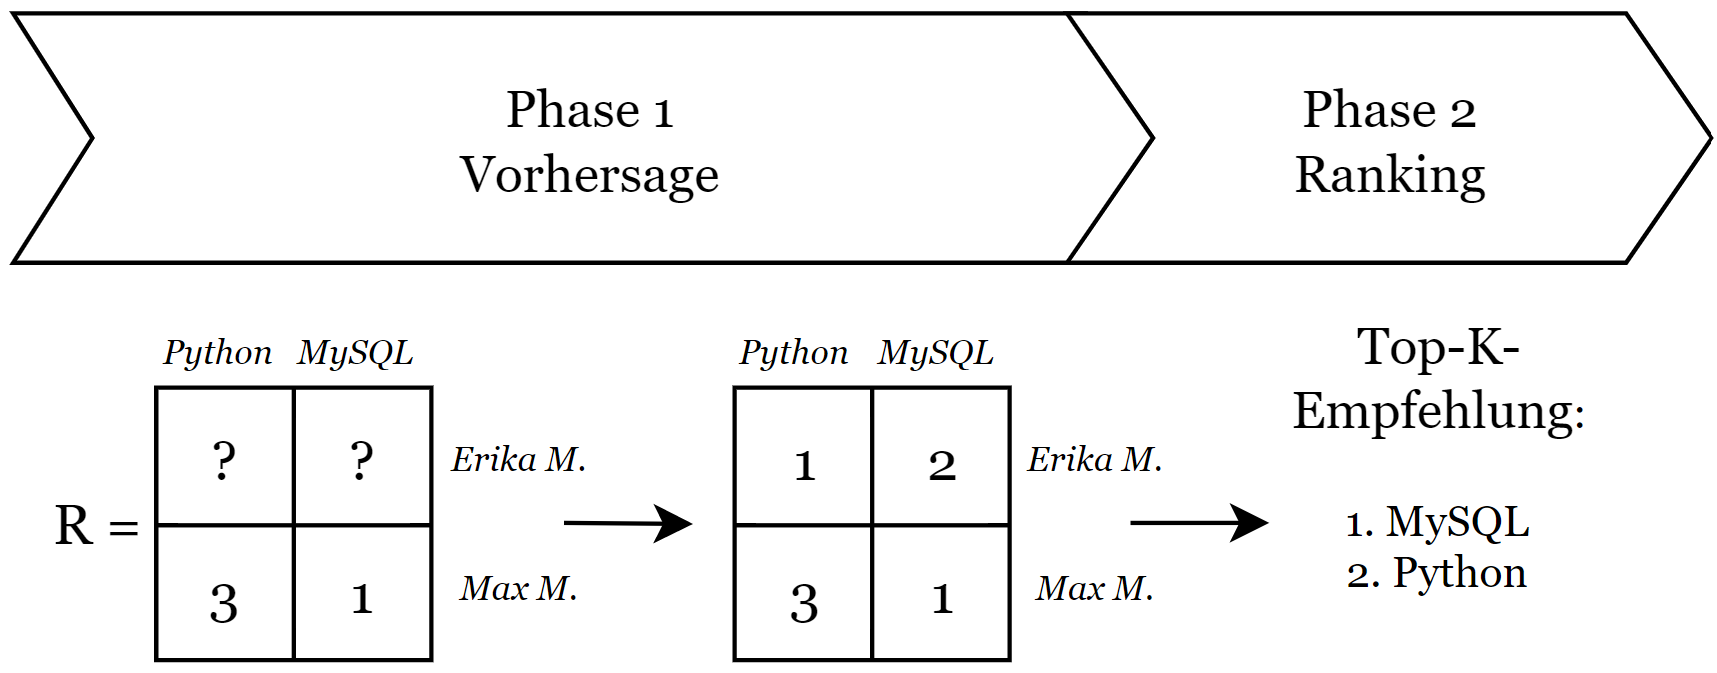
\includegraphics[width=1.0\textwidth]{gfx/phasen-empfehlungserstellung.png}
	\caption[Phasen der Empfehlungserstellung]{Phasen der Empfehlungserstellung\\}
	\label{fig:empfehlungssysteme:recommendation:abb1}
\end{figure}

Empfehlungen dieser Art können beispielsweise sinnvoll sein, wenn Mitarbeitern Fähigkeiten vorgeschlagen werden sollen, die sie verhältnismäßig schnell erlernen können.
% Empfehlungen dieser Art können beispielsweise sinnvoll sein, wenn Mitarbeitern Fähigkeiten vorgeschlagen werden sollen, die viele Ähnlichkeiten zu bereits existierenden Fähigkeiten eines Mitarbeiters aufweisen.
% Dies kann sinnvoll sein, wenn Mitarbeiter möglichst schnell eine Fähigkeit erlernen sollen.
% Wenn angenommen wird, dass Mitarbeiter, die bereits Fähigkeiten besitzen, welche Ähnlichkeiten zu der gefragten Fähigkeit aufweisen, schneller die gefragte Fähigkeit erlernen als Mitarbeiter, die diese Fähigkeiten nicht oder weniger gut beherrschen.
So kann es vorteilhaft sein, der Mitarbeiterin Erika M. die Fähigkeit MySQL für eine Schulung vorzuschlagen, da aufgrund ihrer Vorkenntnisse in MongoDB angenommen werden kann, dass sie sich My\-SQL im Verhältnis zu anderen unbekannten Fähigkeiten wie Python schnell aneignen kann.

\section{Präferenzen in Empfehlungssystemen}
\label{ch:empfehlungssysteme:preferences}
Im Zusammenhang mit Empfehlungssystemen fällt häufig der Begriff der Präferenzen (engl.: preferences) \cite[S. 11f.]{recommenderSystems:2016}\cite[S. 87]{ekstrand:article}\cite[S. 2429]{palomares:inproceedings}\cite[S. 2]{ricci:inbook}.
% Brauch man hier überhaupt ein zitat, wenn ich die Annahme selber aufstelle?
Ein Verständnis der Präferenzen von Nutzern eines Systems kann für die erfolgreiche Ermittlung von Empfehlungen von großer Bedeutung sein. % \cite[S. 1]{jawaheer:article}
In diesem Kapitel werden Präferenzen daher allgemein erläutert und im Kontext von Empfehlungssystemen inhaltlich abgegrenzt.

% Nach dem Verständnis der Bundeszentrale für politische Bildung können Präferenzen grundsätzlich als Vorlieben und Verhaltensweisen von Personen verstanden werden, "[...], die bewirken, dass Güter unterscheidbar werden."\cite{pollert:book}
% Wenn Präferenzen in dem Kontext von Empfehlungssystemen aufkommen, wird sich in der Regel auf die Vorlieben und Verhaltensweisen der Nutzer des Systems bezogen.
% Beispielsweise kann unter der Präferenz eines Nutzers in einem Online-Shop die Bevorzugung eines Produktes gegenüber eines Anderen Verstanden werden.

In der Literatur wird unter Präferenzen eines Nutzers zumeist dessen explizite und / oder implizite Bewertungen von Elementen verstanden \cite[S. 743]{adomavicius:inproceedings}\cite[S. 899]{adomavicius:article}\cite[S. 11]{recommenderSystems:2016}\cite[S. 37]{berkovsky:2:article}\cite[S. 129]{ekstrand:article}.\footnote{Vgl. Kapitel \ref{ch:empfehlungssysteme:nutzenfunktion}.}
Die Präferenz eines Nutzers $c$ für ein Element $s$ kann daher als das (angenommene) Rating $R(c,s)$ verstanden werden.
Die Präferenzen von Nutzern sind jedoch keinesfalls trivial.
Dies hängt unter anderem damit zusammen, dass einer expliziten Bewertung (z.B. einer Gefällt-mir-Angabe in Facebook) durch einen Nutzer aus der Sicht eines Nutzers ein unterschiedlicher Wert zukommen kann als aus Sicht des Systems.
Darüber hinaus kann auch die Bewertungsskala eines Elements Einfluss auf die Genauigkeit von Präferenzen haben.
So kann eine fehlende Gefällt-mir-Angabe für ein Element durch einen Nutzer in Facebook nicht zwangsläufig als Abneigung für das Element verstanden werden \cite[S. 11]{recommenderSystems:2016}.

Anhand von Präferenzen ist es möglich, Empfehlungen für Nutzer eines Empfehlungssystems zu personalisieren.
In Abhängigkeit des Grads der Personalisierung können Empfehlungen personalisierten bzw. nicht-personali\-sierten Empfehlungen zugeordnet werden (in Anlehnung an \cite[S. 400]{unternährer:article}).

\subsection{Personalisierte und nicht-personalisierte Empfehlungen}
\label{ch:empfehlungssysteme:preferences:personal_vs_nonpersonal}
Unter nicht-personalisierten Empfehlungen versteht \textcite[S. 400]{unternährer:article} Empfehlungen, die für alle Nutzer eines Systems gleich sind.
Das bedeutet, alle Nutzer eines Empfehlungssystems bekommen dieselben Elemente vorgeschlagen, unabhängig von ihren Präferenzen oder ihrem Nutzerprofil (z.B. "Top 10 Lieder aller Zeiten").

Für die Ermittlung nicht-personalisierter Empfehlungen können Popularitätsmetriken herangezogen werden.
Dies folgt der Annahme, dass Popularität einen guten Prädiktor der Präferenzen aller Nutzer eines Systems darstellt \cite[S. 406]{unternährer:article}.
Popularitätsmetriken sind sortierte Listen, über die Elemente in ordinale Relationen gesetzt werden können (z.B. Element A ist höher sortiert als Element B, da es einen höheren Rang aufweist) \cite[S. 404ff.]{unternährer:article}.
Die Listen werden basierend auf den "aggregierten Präferenzen" aller Nutzer eines Systems generiert \cite[S. 404]{unternährer:article}.
Hierfür muss im Vorfeld bestimmt werden, welcher Indikator für die Bestimmung der Popularität in einem System geeignet ist (z.B. die Anzahl an Klicks oder Gefällt-mir-Angaben) \cite[S. 406]{unternährer:article}.

Nicht-personalisierte Empfehlungen müssen nicht allein auf absoluter Popularität beruhen.
Nach \textcite[S. 405]{unternährer:article} ermöglichen zeitliche, räumliche und soziale Popularität, absolute Popularität zu begrenzen.
So können Nachrichten-Plattformen beispielsweise gezielt die populärsten Artikel des Tages (zeitliche Popularität) auf ihrer Startseite anzeigen, anstelle der populärsten Artikel aller Zeiten (absolute Popularität).
Unter der Annahme, dass die Relevanz der Beiträge mit deren Aktualität zusammenhängt, kann durch Verwendung von zeitlicher Popularität für die Ermittlung von Empfehlungen die Relevanz von Beiträgen auf der Startseite erhöht werden \cite[S. 405]{unternährer:article}.
% In der Literatur werden nicht-personalisierte Empfehlungen größtenteils vernachlässigt \cite[S. 2]{ricci:inbook}.
% Fragwürdig, ob das nicht auch schon eine art der personalisierung ist? Es ist anzunehmen, dass nicht-personalisiert einfach bedeutet, dass nicht die präfeenzen eines nutzers speziell verwendet werden, um gezielt empfehlungen zu schalten, sondern eben allgemein

Der maßgebende Unterschied zu personalisierten Empfehlungen besteht darin, dass das Erstellen von nicht-personalisierten Empfehlungen für einen Nutzer nicht auf dessen individuellen Präferenzen beruht.
Empfehlungen können somit völlig unabhängig davon erstellt werden, ob ein Nutzer eines Empfehlungssystems bereits eine Interaktion mit einem System aufweist oder nicht.
Dies ermöglicht Systemen auch Empfehlungen für Nutzer zu erstellen, für die keine Präferenzen bekannt sind.
Ausschlaggebend ist lediglich, dass Informationen vorliegen, die es ermöglichen, die Popularität von Elementen zu ermitteln.
So kann beispielsweise kein populärster Artikel des Tages einer Nachrichten-Plattform ermittelt werden, wenn überhaupt keine Interaktionen mit Artikeln des Systems vorliegen.

Personalisierte Empfehlungen stellen Vorschläge dar, die basierend auf individuellen Präferenzen von Nutzern erstellt werden (bspw. über explizite oder implizite Bewertungen).
Der Grad der Personalisierung ermöglicht eine weitere Unterteilung der personalisierten Empfehlungen in schwach- und stark-personali\-sierte Empfehlungen.
Unter schwacher Personalisierung versteht \textcite[S. 407]{unternährer:article} stereotypisierende Empfehlungen, die Nutzer basierend auf deren Attributen (z.B. Wohnort, Alter, Geschlecht) bestimmten Kategorien zuordnen.
Prinzipiell ähneln schwach-personalisierte Empfehlungen den nicht-personalisierten Empfehlungen, da sie auch basierend auf Popularitätsmetriken erstellt werden.
Der Unterschied besteht darin, dass die Popularität von Elementen innerhalb einer Kategorie ermittelt wird.
Die Empfehlungen der populärsten Elemente für einen Nutzer erfolgen dann in Abhängigkeit der kategorialen Zugehörigkeit des Nutzers \cite[S. 407ff.]{unternährer:article}.

Stark-personalisierte Empfehlungen verzichten auf pauschale und kategoriale Vorentscheidungen und beziehen sich für das Ermitteln von Empfehlungen auf paarweise Relationen (sog. "Good Matches") zwischen Nutzern untereinander bzw. zwischen Nutzern und deren Elementen \cite[S. 415]{unternährer:article}.
Solche Sachverhalte sind vorwiegend in Systemen des kollaborativen Filterns und inhaltsbasierten Empfehlungssystemen anzutreffen.
Hierbei werden nicht nur einzelne Nutzer oder Elemente bewertet \cite[S. 417]{unternährer:article}. 
Stattdessen wird der "Fit" einer Kombination an Nutzer und Element bewertet.
Das bedeutet, es wird eine Relation zwischen einem Nutzer und einem Element erstellt, die dann mit anderen Relationen verglichen werden kann.
Beispielsweise kann eine Fünf-Sterne-Bewertung eines Produktes durch einen Nutzer als starker "Fit" des Produktes mit dem Nutzer gesehen werden.
Diese Beziehung zwischen Nutzer und Produkt kann dann mit anderen Beziehungen verglichen werden, um daraus Präferenzen von Nutzern abzuleiten \cite[S. 417]{unternährer:article}.
% Popularitätsmetriken bewerten, wie gut ein element ist und ob es besser oder schlechter als ein anderes ist, während personalisierte empfehlungen beziehungen zwischen nutzern und elementen bewerten

Eine Voraussetzung für das Erstellen personalisierter Empfehlungen ist die Abbildung der Präferenzen der Nutzer eines Systems \cite[S. 36]{berkovsky:2:article}.

\subsection{Zugrundeliegende Datenstruktur}% Frage ist, wie Präferenzen in RS aussehen, erwähnen
\label{ch:empfehlungssysteme:preferences:data}
Präferenzen von Nutzern werden in Empfehlungssystemen über sogenannte Nutzermodelle dargestellt \cite[S. 246]{berkovsky:article}\cite[S. 2]{jawaheer:article}\cite[S. 9]{ricci:inbook}.
Nach \textcite[S. 249f.]{berkovsky:article} speichern Nutzermodelle die Präferenzen traditionell in einer zweidimensionalen Matrix $R'_{gen}$:
\begin{equation}\label{eq4}
    R'_{gen}: Nutzer_{Attribut} \times Element_{Attribut} \rightarrow rating
\end{equation}
Hierbei kennzeichnet die Dimension $Nutzer_{Attribut}$ Attribute der Nutzer (z.B. ID, Name, Geschlecht) und die Dimension $Element_{Attribut}$ Attribute der Elemente (z.B. ID, Produktkategorie, Genre).
Das $rating$ stellt die Bewertungen der Nutzer für Elemente dar \cite[S. 250]{berkovsky:article}.

In Abhängigkeit der eingesetzten Technik innerhalb eines Empfehlungssystems (Vgl. Kapitel \ref{ch:empfehlungssysteme:empfehlungserstellung:prediction}) muss die Matrix $R'_{gen}$ Nutzermodelle mit unterschiedlichen Daten abbilden können. % Zitat? \cite[S. 248]{berkovsky:article}

In Systemen des kollaborativen Filterns werden Präferenzen von Nutzern für Elemente in der Rating-Matrix $R$ gespeichert \cite[S. 246ff.]{berkovsky:article}.
Nutzer und Elemente werden dabei jeweils über ein eindeutiges Attribut (z.B. ID, Name) beschrieben.
Daraus ergibt sich nach \textcite[S. 250]{berkovsky:article} für die Abbildung der Nutzermodelle in Matrix $R_{CF}$ folgende Form:
\begin{equation}\label{eq5}
    R_{CF}: Nutzer_{ID} \times Element_{ID} \rightarrow rating
\end{equation}
Die Dimensionen $Nutzer_{ID}$ und $Element_{ID}$ stellen die eindeutig beschreibenden Attribute der Nutzer und Elemente dar.
Anhand des Beispiels aus Kapitel \ref{ch:empfehlungssysteme:nutzenfunktion} ist in Abbildung \ref{fig:empfehlungssysteme:preferences:abb1:1} ein Beispiel einer Nutzer$_{ID}$$\times$Element$_{ID}$-Matrix abgebildet.\footnote{Für eine bessere Übersicht wurde das Beispiel auf die drei Fähigkeiten Java, Python und MySQL reduziert und die Bewertungen lediglich für einen Beispiel-Mitarbeiter (hier: John D.) angegeben.}
Mitarbeiter und Fähigkeiten werden jeweils eindeutig über deren Namen gekennzeichnet (d.h. Attribut ID = Name).
% Der Sachverhalt wird nachfolgend anhand des Beispiels aus Kapitel \ref{ch:empfehlungssysteme:nutzenfunktion} erläutert.
% Hierfür sind in Abbildung \ref{fig:empfehlungssysteme:preferences:abb1:1} die Nutzermodelle einiger Mitarbeiter des Beispiels in einer Matrix dargestellt.\footnote{Für eine bessere Übersicht wurden das Beispiel auf die drei Fähigkeiten Java, Python und MySQL reduziert und die Bewertungen lediglich für einen Beispiel-Mitarbeiter (hier: John D.) angegeben.}
% \begin{figure}[H]
%     \centering
%     \subfloat[Nutzer$_{ID}\times$Element$_{ID}$ - Matrix]{\includegraphics[height=1.5in]{gfx/abbildung-präferenzen-A.png}\label{fig:empfehlungssysteme:preferences:abb1:1}}\\
%     \subfloat[Nutzer$_{ID}\times$Element$_{Attribut}$ - Matrix]{\includegraphics[height=1.48in]{gfx/abbildung-präferenzen-B.png}\label{fig:empfehlungssysteme:preferences:abb1:2}}\\
%     \subfloat[Nutzer$_{Attribut}\times$Element$_{Attribut}\times$Kontext$_{Attribut}$ - Matrix]{\includegraphics[height=1.85in]{gfx/abbildung-präferenzen-C.png}\label{fig:empfehlungssysteme:preferences:abb1:3}}
%   \caption[Abbildung von Präferenzen]{Abbildung von Präferenzen\\
% 	(Eigene Darstellung in Anlehnung an \cite[S. 198]{adomavicius:3:inbook})}\label{fig:empfehlungssysteme:preferences:abb1}
% \end{figure}
% Werden Nutzermodelle in Systemen folglich über eine Nutzer$\times$Element-Matrix abgebildet, können die Präferenzen eines Nutzers unmittelbar aus der Rating-Matrix abgelesen werden.

\begin{figure}[H]
    \centering
	\includegraphics[width=1.1\textwidth]{gfx/abbildung-präferenzen-A.png}
	\caption[Abbildung von Präferenzen in Systemen des kollaborativen Filterns]{Abbildung von Präferenzen in Systemen des kollaborativen Filterns}
	\label{fig:empfehlungssysteme:preferences:abb1:1}
\end{figure}

Ein Nutzermodell $UM_{c}$ entspricht genau einer Sammlung aller Bewertungen eines Nutzers $c$ dieser Matrix.
Nach \textcite[S. 41]{berkovsky:2:article} kann diese Sammlung beispielsweise als Liste paarweiser Einträge dargestellt werden:
\begin{equation}\label{eq6}
    UM_{c} = \{s_{1}:r_{1},\textnormal{ }s_{2}:r_{2},\textnormal{ }...,\textnormal{ }s_{k}:r_{k}\}
\end{equation}
Dabei stellt jedes Paar $s_{j}:r_{j}$ die Bewertung $r_{j}$ eines Elements $s_{j}$ durch den Nutzer $c$ dar \cite[S. 41]{berkovsky:2:article}.
Daraus ergibt sich beispielsweise für den Nutzer John D. das Nutzermodell $UM_{John\textnormal{ }D.} = \{Java: 3, Python:\textnormal{ ?}, MySQL: 2\}$ (Vgl. Abbildung \ref{fig:empfehlungssysteme:preferences:abb1:1}).

Ein Vergleich der Matrix $R_{CF}$ aus Abbildung \ref{fig:empfehlungssysteme:preferences:abb1:1} mit der Rating-Matrix aus Tabelle \ref{tab1} zeigt, dass Abbildung \ref{fig:empfehlungssysteme:preferences:abb1:1} lediglich einen vereinfachten Ausschnitt der Rating-Matrix darstellt.
In Systemen des kollaborativen Filterns sind die Nutzer$_{ID}$$\times$Element$_{ID}$-Matrix zur Abbildung der Nutzermodelle und die Rating-Matrix folglich identisch.

In inhaltsbasierten Empfehlungssystemen stellen nicht die Bewertungen der Nutzer für Elemente als Ganzes deren Präferenzen dar, sondern die Bedeutung einzelner Elementattribute für einen Nutzer.
Nutzermodelle müssen folglich nicht die Bewertungen von Nutzern für Elemente, sondern die Wichtigkeit einzelner Elementattribute für einen Nutzer darstellen \cite[S. 42]{berkovsky:2:article}.
Nach \textcite[S. 42]{berkovsky:2:article} entspricht ein Nutzermodell demnach einer Sammlung der Wichtigkeiten (meist in Form von Gewichten) einzelner Elementattribute für einen Nutzer.
Ein solches Nutzermodell lässt sich ebenfalls als eine Liste paarweiser Einträge abbilden:
\begin{equation}\label{eq7}
    UM_{c} = \{a_{1}:w_{a(1)}, a_{2}:w_{a(2)}, ..., a_{k}:w_{a(k)}\}
\end{equation}
Jedes Paar $a_{j}:w_{a(j)}$ stellt das Gewicht $w$ eines Elementattributs $a$ für den Nutzer $c$ dar \cite[S. 42]{berkovsky:2:article}.
Für die Darstellung der Nutzermodelle eines inhaltsbasierten Systems ergibt sich nach \textcite[S. 251]{berkovsky:article} folgende Matrix:
\begin{equation}\label{eq8}
    R_{CB}: Nutzer_{ID} \times Element_{Attribut} \rightarrow rating
\end{equation}
Hierbei umfasst Element$_{Attribut}$ das Attribut, durch das die Elemente eines Systems beschrieben werden können \cite[S. 251]{berkovsky:article}.

Abbildung \ref{fig:empfehlungssysteme:preferences:abb1:2} illustriert eine solche Nutzer$_{ID}$$\times$Element$_{Attribut}$-Matrix anhand des Beispiels aus Kapitel \ref{ch:empfehlungssysteme:nutzenfunktion}.

\begin{figure}[H]
    \centering
	\includegraphics[width=1.1\textwidth]{gfx/abbildung-präferenzen-B.png}
	\caption[Abbildung von Präferenzen in inhaltsbasierten Systemen]{Abbildung von Präferenzen in inhaltsbasierten Systemen}
	\label{fig:empfehlungssysteme:preferences:abb1:2}
\end{figure}

Als Elementattribut wurde für dieses Beispiel die Typisierung einer Programmiersprache mit den Ausprägungen "Statisch" und "Dynamisch" gewählt.
Ein Nutzermodell enthält für alle Ausprägungen des Attributs Gewichte $w$, die den Wert eines Elementattributs für einen Nutzer abbilden \cite[S. 251]{berkovsky:article}.
Daraus ergibt sich beispielsweise für den Nutzer John D. das Nutzermodell $UM_{John\textnormal{ }D.} = \{Statisch:\textnormal{ 1.0}, Dynamisch: \textnormal{ 0.0}\}$ (Vgl. Abbildung \ref{fig:empfehlungssysteme:preferences:abb1:2}).

Um die Gewichte einer Nutzer$_{ID}$$\times$Element$_{Attribut}$-Matrix zu ermitteln, existieren in der Literatur verschiedene Verfahren \cite[S. 42]{berkovsky:2:article}.
Grundsätzlich wird die Nutzer$_{ID}$$\times$Element$_{Attribut}$-Matrix auf Basis der Rating-Matrix generiert.
Bei den Gewichten in Abbildung \ref{fig:empfehlungssysteme:preferences:abb1:2} handelt es sich lediglich um ein willkürliches Beispiel, da der Fokus dieses Kapitels auf der Darstellung der Präferenzen und nicht auf den Verfahren für die Ermittlung der Attributgewichte liegt.

Neben der traditionellen Darstellung der Präferenzen von Nutzern in einem zweidimensionalen Raum, können Präferenzen auch in dreidimensionaler Form abgebildet werden.
Diese Darstellung beruht auf der Annahme, dass Präferenzen von Nutzern für Elemente zusätzlich durch kontextuelle Information (z.B. Zeit, Ort, Gesellschaft) beeinflusst werden \cite[S. 195]{adomavicius:3:inbook}.
% Eine zweidimensionale Darstellung der Präferenzen wie in Gleichung \ref{eq4} vernachlässigt demnach eine entscheidende Dimension: den Kontext von Präferenzen \cite[S. 253]{berkovsky:article}.
Für die Darstellung der Nutzermodelle wird daher in kontextbasierten Empfehlungssystemen von einer Matrix $R_{CA}$ ausgegangen \cite[S. 254]{berkovsky:article}:
\begin{equation}\label{eq9}
    R_{CA}: Nutzer_{Attribut} \times Element_{Attribut} \times Kontext_{Attribut} \rightarrow rating
\end{equation}
Matrix $R_{CA}$ erweitert die zweidimensionale Darstellung aus Gleichung \ref{eq4} um die Dimension $Kontext_{Attribut}$, welche den Kontext einer Bewertung angibt \cite[S. 254]{berkovsky:article}.\footnote{\textcite[S. 249ff.]{berkovsky:article} merken an, dass es sich bei den Dimensionen $Nutzer_{Attribut}$ und $Element_{Attribut}$ auch um Sammlungen von Attributen handeln kann. Dies ist der Fall, wenn Nutzer oder Elemente für das Abbilden von Präferenzen über mehrere Attribute beschrieben werden. Angenommen die Präferenzen von Nutzern können über $n$ Attribute des Nutzers und $m$ Attribute der Elemente ($n \cup m > 1$) beschrieben werden, so ergibt sich für $R'_{gen}$ eine multidimenisonale $n+m$-Matrix. Dies gilt analog für die Dimension $Context_{Attribut}$ \cite[S. 254f.]{berkovsky:article}.}
% MIT AUFNEHMEN JA/ NEIN?
% In Anlehnung an \textcite[S. 250ff]{berkovsky:article} und \textcite[S. 198]{adomavicius:3:inbook} kann für die Abbildung der zugehörigen Nutzermodelle Liste an Tripeln angenommen werden:
% \begin{equation}\label{eq10}
%     UM_{c} = \{(s_{1},q_{1}):r_{1},\textnormal{ }(s_{2},q_{2}),\textnormal{ }...,\textnormal{ }(s_{k},q_{k})\}
% \end{equation}
% Jeder Eintrag $(s_{k},q_{k}):r_{k}$ in $UM_{c}$ stellt die Bewertung eines Nutzers $c$ für ein Element

Eine dreidimensionale Darstellung von Nutzermodellen ist beispielhaft in Abbildung \ref{fig:empfehlungssysteme:preferences:abb1:3} dargestellt.

\begin{figure}[H]
    \centering
	\includegraphics[width=1.0\textwidth]{gfx/abbildung-präferenzen-C.png}
	\caption[Multidimensionale Abbildung von Präferenzen]{Multidimensionale Abbildung von Präferenzen\\
    (Eigene Darstellung in Anlehnung an \cite[S. 198]{adomavicius:3:inbook})}
	\label{fig:empfehlungssysteme:preferences:abb1:3}
\end{figure}

Die abgebildete Nutzer$_{ID}$$\times$Element$_{ID}$$\times$-Kontext$_{ID}$-Matrix stellt eine Erweiterung der Matrix aus Abbildung \ref{fig:empfehlungssysteme:preferences:abb1:1} um die kontextuelle Information "Teamzugehörigkeit" dar.
Dem liegt die Annahme zugrunde, dass die Einschätzung der eigenen Fähigkeiten eines Mitarbeiters von den Teamkollegen abhängt, mit denen er zusammenarbeitet.
Folglich kann ein Mitarbeiter für eine Fähigkeit mehrere Bewertungen aufweisen.

Ein Eintrag $R_{CA}(c_{i},s_{j},q_{t}) = r_{ijt}$ der Matrix stellt die Bewertung $r_{ijt}$ einer Fähigkeit $s_{j}$ durch einen Mitarbeiter $c_{i}$ innerhalb eines Teams $q_{t}$ dar \cite[S. 198]{adomavicius:3:inbook}.
Folglich repräsentiert ein Nutzermodell eine Sammlung aller Bewertungen von Fähigkeiten durch einen Mitarbeiter in Abhängigkeit der Teamzugehörigkeit.
Ein Beispiel eines Nutzermodells $UM$ unter Berücksichtigung des Kontextes ist anhand des Mitarbeiters John D. in Abbildung \ref{fig:empfehlungssysteme:preferences:abb1:3} dargestellt.
% Die angegebenen Bewertungen sind willkürlich gewählt.
% Hier was anderes als Teamzugehörigkeit finden! das macht in dem kontext keinen sinn

% Bei popularität: nur bewertung von element ist ausschlaggeben, ggf. noch kategorie, aber sonst reicht bewertung, um ordinale Relation zu erstellen -> d.h. über alle nutzer verteilt die durchschnittlich höchste bewertung -> es existieren nicht wirklich individuelle präferenzen, eher ableitung aus aggregierten präferenzen
% Bei paarweiser Relation: Bewertung einer Beziehung, d.h. betrachten von beziehungen zwischen Nutzern und Elementen, bzw. sogar zwischen Nutzer und Nutzern -> präferenz bedeutet hier die ordinale ordnung von elementen für einen Nutzer (hier habe ich leider keine referenz zu literatur, lediglich eine annahme, muss also weiterschauen)
% das ist der wichtige unterschied zu uns, da wir präferenzen als ein attribut des mitarbeiters bzw als ein attribut des nutzers verstehen, und nicht als interpretation einer relation
\section{Wechselseitige Empfehlungssysteme}
\label{ch:empfehlungssysteme:rrs}
% Problem: ist reciprocal recommender nur, wenn das empfehlende element auch selber entscheidet, wen es annimmt?
% Nach \textcite[S. 2429]{palomares:inproceedings} werden Empfehlungssysteme größtenteils in Online-Diensten eingesetzt, um Nutzern basierend auf ihren (expliziten oder impliziten) Präferenzen potenziell interessante Elemente vorzuschlagen.
% Zu klassischen Inhalten von Empfehlungen zählt \textcite[S. 2429]{palomares:inproceedings} Objekte wie Musik, Filme, Konsumgüter und Restaurants. 
 
% Als wechselseitig werden Empfehlungssysteme bezeichnet, in denen Personen den Inhalt von Empfehlungen bilden und für die Empfehlungserstellung sowohl die Präferenzen der Empfänger, als auch der empfohlenen Personen berücksichtigt werden (bspw. in Online-Dating-Plattformen oder Recruiting-Systemen) \cite[S. 35]{li:inproceedings}\cite[S. 2199]{akehurst:inproceedings}\cite[S. 207]{pizzato:2010}.
Empfehlungssysteme, in denen Personen die Inhalte von Empfehlungen bilden und diese Empfehlungen reziprok sind, werden in der Literatur als wechselseitige Empfehlungssysteme (engl.: \ac{RRS}) bezeichnet \cite[S. 2199]{akehurst:inproceedings}\cite[S. 35]{li:inproceedings}\cite[S. 207]{pizzato:2010}.
Reziprok bedeutet, dass für eine erfolgreiche Empfehlung sowohl die Präferenzen des Empfängers einer Empfehlung, als auch die Präferenzen der empfohlenen Person berücksichtigt werden \cite[S. 22]{kleinerman:inproceedings}\cite[S. 447]{pizzato:2013}.
Der Erfolg einer Empfehlung ist demnach von den bilateralen Präferenzen abhängig.
In der Literatur sind wechselseitige Empfehlungssysteme daher auch als bilaterale Empfehlungssysteme bekannt \cite[S. 32]{link:booklet}.
Analog werden Systeme, die lediglich die Bedürfnisse der Empfehlungsempfänger berücksichtigen als unilaterale Systeme bezeichnet.
Bekannte Domänen für den Einsatz wechselseitiger Empfehlungssysteme sind Online-Dating und (semi-)automatisiertes Recruiting.
Nachfolgend wird das Konzept der \ac{RRS} und dessen zugrundeliegende Problemstellung erläutert.

\subsection{People-to-People-Empfehlungen}% oder umbenennen in Allgemeines Konzept
\label{ch:empfehlungssysteme:rrs:people_to_people}
Ein grundlegender Unterschied zwischen klassischen Empfehlungssystemen und \ac{RRS} liegt in der Art der Empfehlung.
Diese können in \ac{I2P}- und \ac{P2P}-Empfehlungen unterschieden werden \cite[S. 62f.]{kim:inproceedings}.

In der Literatur wird unter traditioneller \ac{I2P}-Empfehlung die Empfehlung klassischer Inhalte (z.B. Bücher, Filme, Hotels) verstanden \cite[S. 2199]{akehurst:inproceedings}\cite[S. 2429]{palomares:inproceedings}.
In \ac{I2P}-Empfehlungen ist der Erfolg einer Empfehlung durch die Akzeptanz des Empfehlungsempfängers (d.h. des Nutzers) gekennzeichnet \cite[S. 131]{kleinerman:2:inproceedings}\cite[S. 546]{koprinska:inbook}.
% Für personalisierte \ac{I2P}-Empfehlungen verwenden Empfehlungssysteme Wissen über die Präferenzen der Nutzer, um ihnen potenziell interessante Elemente zu empfehlen \cite[S. 403]{terveen:article}.

% Ein grundlegendes Problem, welches dieser Art der Empfehlung löst, ist das Problem der Informationsüberlastung \cite[S. 403]{terveen:article}.
% Indem Empfehlungssysteme Nutzern aus einem Überangebot an (unbekannten) Elementen potenziell nützliche Elemente vorschlagen, können sie Nutzer bei der Entscheidungsfindung unterstützen.

Im Vergleich zu traditionellen Empfehlungssystemen basieren \ac{RRS} auf \ac{P2P}-Empfehlungen \cite[S. 207]{pizzato:2010}.
Unter \ac{P2P}-Empfehlung (auch: social matching \cite[S. 208]{pizzato:2010}) wird die Empfehlung von Personen an Nutzer eines Empfehlungssystems verstanden.
Im Gegensatz zu \ac{I2P}-Empfehlungen, handelt es sich bei den empfohlenen Elementen nicht um leblose Objekte, sondern um Menschen, die anderen Menschen empfohlen werden \cite[S. 2]{kazienko:inbook}.
Das bedeutet, dass auch die empfohlenen Elemente Präferenzen besitzen und auch positiv oder negativ reagieren können \cite[S. 2]{kazienko:inbook}.
Dies ist ein besonderer Aspekt, den es zu beachten gilt, da dadurch die Qualität der Empfehlungen beeinflusst werden kann \cite[S. 208]{pizzato:2010}\cite[S. 2199]{akehurst:inproceedings}.

Während ein Großteil der \ac{P2P}-Empfehlungen auf dem Aspekt der Reziprozität (engl.: reciprocity) beruhen \cite[S. 545]{koprinska:inbook}, ist nicht jede \ac{P2P}-Empfehlung unmittelbar reziprok.
Empfehlungen können auch \ac{P2P}-Empfehlungen sein und lediglich die Präferenzen des Nutzers berücksichtigen \cite[S. 2429]{palomares:inproceedings}.
Ein Beispiel stellen \ac{P2P}-Empfehlungen des sozialen Netzwerks Twitter dar \cite[S. 2429]{palomares:inproceedings}.
Der Vorschlag einer anderen Person zu folgen beruht dabei lediglich auf den Präferenzen des Empfängers des Vorschlags.

\subsection{Abgrenzung traditioneller Empfehlungssysteme}
\label{ch:empfehlungssysteme:rrs:traditional_vs_rrs}
Bei Empfehlungen in \ac{RRS} handelt es sich um reziproke \ac{P2P}-Empfehlungen \cite[S. 207]{pizzato:2010}, deren Erfolg von der Berücksichtigung der bilateralen Präferenzen abhängt.
Im Gegensatz dazu beeinflussen in traditionellen Systemen lediglich die Präferenzen der Nutzer den Erfolg einer Empfehlung \cite[S. 1468]{yildirim:article}.
So reicht es beispielsweise in einem Recruiting-System nicht aus, lediglich die Präferenzen eines Akteurs (bspw. dem Recruiter) zu berücksichtigen.
Damit dem Recruiter auch Personen vorgeschlagen werden, die ein potenzielles Angebot annehmen würden, müssen die Präferenzen der Stellensuchenden ebenfalls in Betracht gezogen werden.
Andernfalls besteht ein erhöhtes Risiko, dass einem Recruiter Stellensuchende vorgeschlagen werden, die aufgrund ihrer Präferenzen ein Angebot des Recruiters ablehnen.

Neben dem Aspekt der Reziprozität besitzen \ac{RRS} zusätzliche Eigenschaften, welche diese im Vergleich zu traditionellen Empfehlungssystemen inhärent komplex machen \cite[S. 2429]{palomares:inproceedings}\cite[S. 35]{li:inproceedings}\cite[S. 207]{pizzato:2010}.
Die wichtigsten Unterschiede zwischen \ac{RRS} und traditionellen \ac{RS} sind in Tabelle \ref{tab2} zusammengefasst \cite[S. 546]{koprinska:inbook}.

\begin{table}[htbp]
    \begin{center}
        \begin{tabular}{|p{0.2\textwidth}||p{0.35\textwidth}|p{0.35\textwidth}|}
            \hline
             & {\textbf{Traditionelle \ac{RS}}} & {\textbf{Wechselseitige \ac{RS}}} \\
            \hline
            \hline
            Reziprozität & Erfolg einer Empfehlung ist durch den Empfänger bestimmt. &  Erfolg einer Empfehlung ist sowohl durch den Empfänger als auch der empfohlenen Person bestimmt. \\
            \hline
            Passivität & Es wird akzeptiert, dass einige Elemente nicht Teil von Empfehlungen sind. &  Auch reaktive Nutzer müssen Teil von Empfehlungen sein. \\
            \hline
            Rolle der Nutzerprofile & Kein Anreiz für Nutzer zum Pflegen des Nutzerprofils. &  Das Pflegen von Nutzerprofilen wird erwartet. \\
            \hline
            Endlichkeit & Ein Element kann allen Nutzern vorgeschlagen werden. & Beliebte Personen sollten nicht allen Nutzern vorgeschlagen werden. \\
            \hline
    \end{tabular}
    \end{center}
    \caption[Grundlegende Unterschiede von RS und RRS]{Grundlegende Unterschiede von RS und RRS \\
	(Eigene Darstellung in Anlehnung an \cite[S. 546]{koprinska:inbook} und \cite[S. 35f.]{li:inproceedings})}
	\label{tab2}
\end{table}

Im Vergleich zu traditionellen Empfehlungssystemen ist die Berücksichtigung der Passivität von Nutzern in einigen \ac{RRS} von großer Bedeutung \cite[S. 35]{li:inproceedings}.
Dies betrifft \ac{RRS}, in denen Nutzer eines Systems sowohl Empfänger von Empfehlungen, als auch empfohlene Elemente desselbigen Systems darstellen (z.B. im Online-Dating).
Zu der Berücksichtigung der Passivität zählt hauptsächlich, reaktive Nutzer in Empfehlungen einzubeziehen, die nicht aktiv den Kontakt zu anderen Nutzern suchen \cite[S. 459]{pizzato:2013}.
Reaktive Nutzer tendieren dazu auf den Kontakt von anderen Nutzern zu warten und nicht selbstständig Kontakte zu suchen \cite[S. 455]{pizzato:2013}.
In \ac{RRS} stellen sie daher hauptsächlich empfohlene Elemente dar, anstatt die Empfänger von Empfehlungen.
Werden reaktive Elemente nicht in Empfehlungen eines Systems inkludiert, besteht das Risiko, dass diese nie mit anderen Nutzern Kontakte eingehen und langfristig das System verlassen \cite[S. 35]{li:inproceedings}.
Im Vergleich dazu können traditionelle Empfehlungssysteme durchaus über inaktive Elemente verfügen, das heißt Elemente, die in keinen Empfehlungen vorkommen \cite[S. 208]{pizzato:2010}.

Nutzer traditioneller Empfehlungssysteme haben in der Regel wenig Anreiz ihre Nutzerprofile zu pflegen \cite[S. 546]{koprinska:inbook}.
Explizite Angaben sind daher meist rar.
Währenddessen verwenden Nutzer traditioneller Systeme diese meist über einen längeren Zeitraum, weshalb der Anteil impliziter Präferenzen verhältnismäßig groß ist \cite[S. 208]{pizzato:2010}.
In \ac{RRS} ist das Pflegen eines Nutzerprofils mit Präferenzen und persönlichen Daten meist fester Bestandteil.
% Nutzern ist bekannt, dass die Nutzerprofile Einfluss auf die generierten Empfehlungen des Systems haben .
Daher sind Nutzer in \ac{RRS} eher gewillt Angaben zu machen \cite[S. 208]{pizzato:2010}.
Es gilt jedoch zu beachten, dass die angegebenen Präferenzen nicht zwangsläufig der Realität entsprechen \cite[S. 457]{pizzato:2013}.
Dies kann unter anderem daran liegen, dass Nutzer diese selbst falsch einschätzen \cite[S. 457]{pizzato:2013}.

In wechselseitigen Empfehlungssystemen sind Empfehlungen für Nutzer endlich.
Das bedeutet, dass ein Element nicht unbegrenzt Nutzern eines Systems vorgeschlagen werden kann.
So ist es unwahrscheinlich, dass ein Nutzer einer Online-Dating-Plattform zeitgleich fünfzig verschiedene Personen kennenlernt \cite[S. 35]{li:inproceedings}.
Diese Eigenschaft wird als Endlichkeit bezeichnet \cite[S. 35]{li:inproceedings}.
Im Vergleich dazu sind Elemente in traditionellen Empfehlungssystemen für Empfehlungen an unterschiedliche Nutzer nicht begrenzt \cite[S. 1468]{yildirim:article}.
Das bedeutet, ein Element kann zeitgleich jedem Nutzer eines Systems vorgeschlagen werden.
% Weiterer unterschied: \ac{RRS} unterstützen keine n-to-n connections % S. 423, https://link.springer.com/content/pdf/10.1007/978-1-0716-2197-4.pdf

\subsection{Problemstellung}\label{ch:empfehlungssyteme:rrs:problem}
Nach \textcite[S. 35]{li:inproceedings} stellt das Zufriedenstellen der Präferenzen beider Akteure, das heißt von sowohl Empfänger einer Empfehlung als auch empfohlener Person, die größte Herausforderung wechselseitiger Systeme dar.
Das Problem ist nachfolgend in Abbildung \ref{fig:empfehlungssysteme:rrs:abb1} veranschaulicht.\footnote{Es gilt zu beachten, dass in \ac{RRS} die Elemente von Empfehlungen (empfohlene Personen) gleichzeitig auch Nutzer desselbigen Systems darstellen können.}
Hierfür wurde die vereinfachte Darstellung des Empfehlungssystems aus Abbildung \ref{fig:empfehlungssysteme:einführung:abb1} aufgegriffen.

Auf der linken Seite ist ein traditionelles Empfehlungssystem dargestellt.
Elemente, die die Bedürfnisse des Nutzers $X$ erfüllen, sind durch einen empfangenden roten Pfeil gekennzeichnet.
Fehlende Verbindungen zwischen Elementen und dem Nutzer $X$ bedeuten, dass ein Element die Präferenzen des Nutzers $X$ nicht erfüllt.
Soll dem Nutzer $X$ das Element empfohlen werden, welches seine Bedürfnisse am stärksten erfüllt, würde nach Abbildung \ref{fig:empfehlungssysteme:rrs:abb1} eindeutig Element $C$ ausgewählt werden.

Auf der rechten Seite von Abbildung \ref{fig:empfehlungssysteme:rrs:abb1} ist ein wechselseitiges Empfehlungssystem vereinfacht dargestellt.
Zusätzlich zu den präferierten Elementen des Nutzers $X$ sind in der Darstellung auch die Präferenzen der empfohlenen Personen abgebildet.
Daraus wird ersichtlich, dass Person $C$ die Präfernezen des Nutzers $X$ erfüllt, aber eine Empfehlung von Person $C$ für Nutzer $X$ nicht die Präferenzen von Person $C$ erfüllen würde.
Eine Empfehlung von Person $A$ würde die Bedürfnisse von Person $A$ erfüllen, dann jedoch die Präferenzen des Nutzers $X$ unerfüllt lassen.
Das Problem besteht folglich darin, aus einer Menge an Personen eine passende Person für Nutzer $X$ zu ermitteln, sodass sowohl die Präferenzen des Nutzers als auch der empfohlenen Person möglichst optimal erfüllt werden.

\begin{figure}[H]
    \centering
	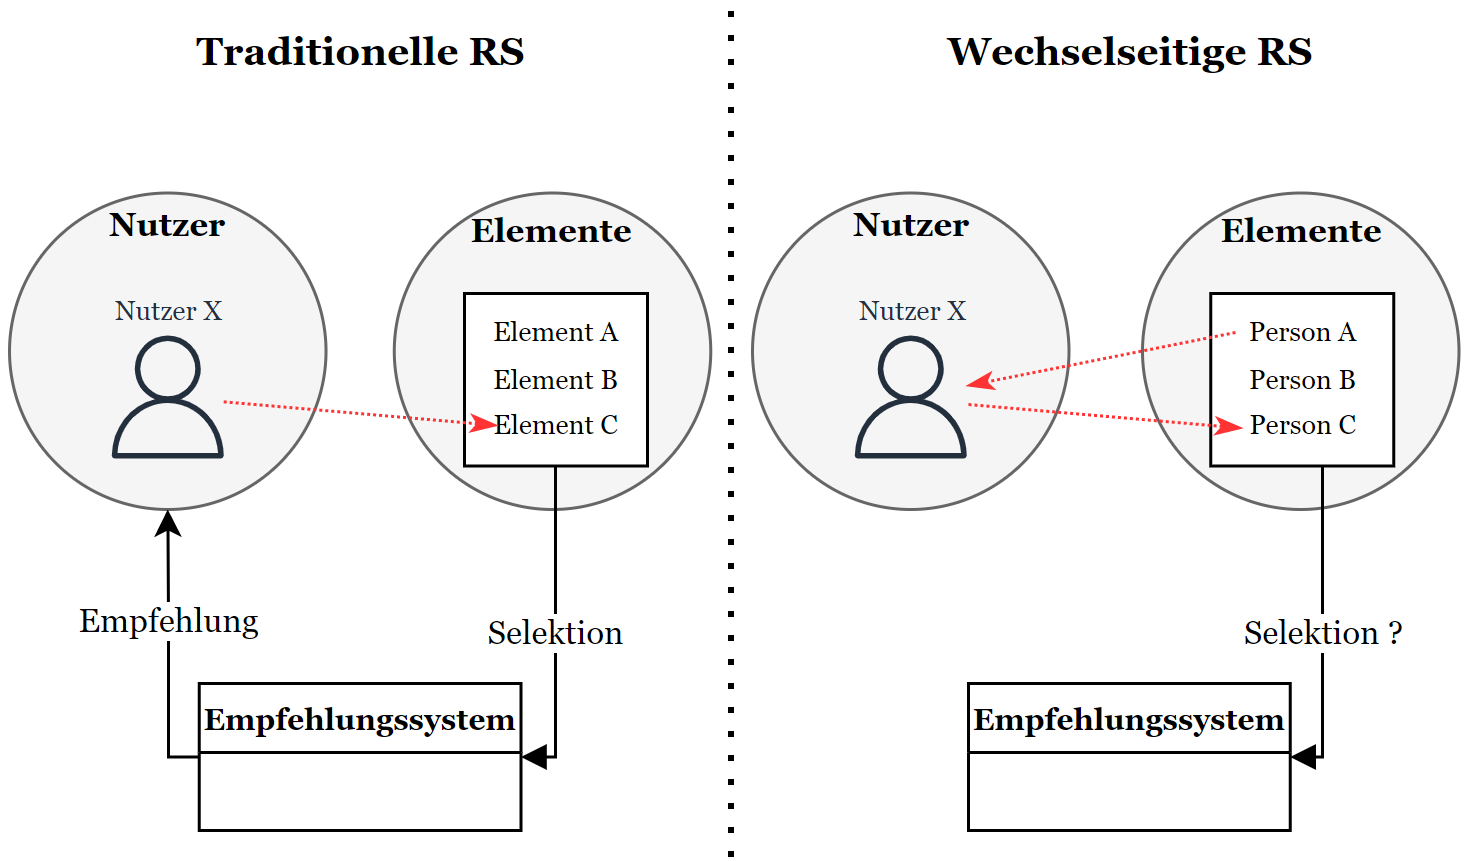
\includegraphics[width=1.0\textwidth]{gfx/traditional-vs-rrs.png}
	\caption[Traditionelle vs. wechselseitige Empfehlungssysteme]{Traditionelle vs. wechselseitige Empfehlungssysteme\\}
	\label{fig:empfehlungssysteme:rrs:abb1}
\end{figure}

Nach \textcite[S. 36]{li:inproceedings} kann diese Problemstellung der reziproken Empfehlung mathematisch als das "Stable Marriage"-Problem modelliert werden.
Das "Stable-Marriage"-Problem beschreibt das Problem der Bestimmung einer optimalen Paarung (engl.: Match) zweier Mengen an Elementen anhand ihrer Präferenzen, sodass kein Element durch Paarung mit einem anderen Partner besser gestellt wäre \cite[S. 36]{li:inproceedings}\cite[S. 67]{diaz:inproceedings}.

Um in dem Szenario einer reziproken Empfehlung zu ermitteln, ob ein Paar optimal ist, müssen nach \textcite[S. 36]{li:inproceedings} für jeden Nutzer $c \in C$ eine Selbstbeschreibung $F_{c}^{d}$ und Präferenzen $F_{c}^{p}$ bekannt sein.
Analog müssen für jede Person (Element) $s \in S$ des Systems eine Selbstbeschreibung $F_{s}^{d}$ und Präferenzen $F_{s}^{p}$ bekannt sein.
Eine optimale Paarung definieren \textcite[S. 36]{li:inproceedings} wie folgt: 

\begin{definition}[Optimale Paarung]\label{def:1}
    Sei ein Nutzer $c \in C$ und eine Person (Element) $s \in S$ gegeben, dann ist das Paar $(c,s)$ optimal, wenn $F_{c}^{d}$ maximal $F_{s}^{p}$ und $F_{s}^{d}$ maximal $F_{c}^{p}$ erfüllt.
\end{definition}

Für reziproke Empfehlungen wird meist kein hartes Match zwischen Nutzer und Element gesucht, sondern eine sortierte Liste an potenziellen Partnern für einen Nutzer \cite[S. 67]{diaz:inproceedings}.
Das heißt, das Ziel der Empfehlungserstellung an einen Nutzer $c$ besteht darin, dem Nutzer eine Liste $L_{s} \subset S$ an Personen $s$ zu empfehlen, sodass die Präferenzen $F_{s}^{p}$ und $F_{c}^{p}$ erfüllt sind \cite[S. 36]{li:inproceedings}.

Das grundlegende Konzept für die Ermittlung des Wertes einer Paarung ist in Abbildung \ref{fig:empfehlungssysteme:rrs:abb2} dargestellt.

\begin{figure}[H]
    \centering
	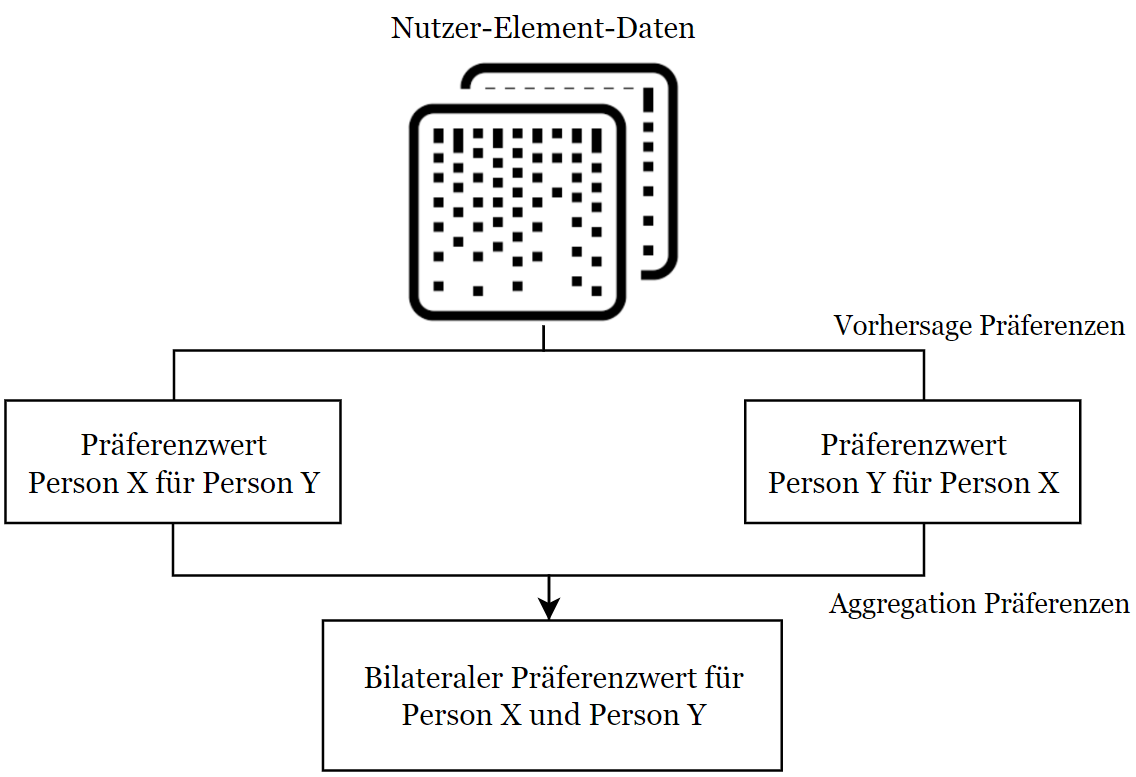
\includegraphics[width=1.0\textwidth]{gfx/concept-rrs.png}
	\caption[Konzept wechselseitiger Empfehlungen]{Konzept wechselseitiger Empfehlungen\\
    (Eigene Darstellung in Anlehnung an \cite[S. 2429]{palomares:inproceedings})}
	\label{fig:empfehlungssysteme:rrs:abb2}
\end{figure}

Nach \textcite[S. 2429]{palomares:inproceedings} werden basierend auf Daten zu Nutzern und Elementen die Präferenzen der Personen füreinander vorhergesagt (d.h. die Erfüllung von $F_{s}^{p}$ und $F_{c}^{p}$).
Die unabhängig voneinander ermittelten Präferenzwerte werden dann mittels Aggregation zu einer Angabe zusammengeführt, welche den angenommenen Wert der bilateralen Paarung angibt.

Nach \textcite[S. 36]{li:inproceedings} ist das Bestimmen einer optimalen Paarung in \ac{RRS} erschwert, da neben der Reziprozität auch Eigenschaften wie die Verfügbarkeit von Elementen (Endlichkeit) berücksichtigt werden müssen.
So kann es sein, dass eine Person anhand ihrer Präferenzen optimal zu einem Nutzer passt, die empfohlene Person aber in einem gegebenen Zeitraum nicht verfügbar ist.
Um dies bei der Bestimmung von Paaren zu berücksichtigen, unterscheiden \textcite[S. 37]{li:inproceedings} daher zusätzlich zwischen optimalem und erfolgreichem Match von Nutzern und Elementen.
Eine erfolgreiche Paarung definieren \textcite[S. 37]{li:inproceedings} wie folgt:

\begin{definition}[Erfolgreiche Paarung]\label{def:2}
    Sei ein Nutzer $c \in C$ und eine Person (Element) $s \in S$ gegeben, dann ist ein Paar $(c,s)$ erfolgreich, wenn $F_{c}^{d}$ suboptimal $F_{s}^{p}$ und $F_{s}^{d}$ suboptimal $F_{c}^{p}$ erfüllt, unter Berücksichtigung der Verfügbarkeit von $c$ und $s$.
\end{definition}

Demnach kann eine Paarung auch dann erfolgreich sein, wenn Beschreibungen von Nutzern bzw. Elementen die Präferenzen des Partners nur teilweise erfüllen \cite[S. 37]{li:inproceedings}.
Dafür können andere Aspekte wie die Verfügbarkeit von Personen in einer erfolgreichen Paarung berücksichtigt werden.

% Hier Überleitung finden zu Multi-kriterieller Optimierung in RS (Anknüpfen über Nutzen, der sich aus mehreren Aspekten zusammensetzt (hier: Nutzen setzt sich zusammen aus Präferenzen Manager und Präferenzen Mitarbeiter)).
% Grundsätzlich basiert das Rating eines Elements auf einem Kriterium.
% Für reziproke Empfehlungen sowohl die Präferenzen der Nutzer als auch die Präferenzen der Elemente berücksichtigt werden müssen.
% Irgendwo noch einbringen, dass Paarung quasi den Nutzen angibt, also gutes paar = guter Nutzen
% Nach \textcite[S. 36]{li:inproceedings} ist eine optimale Paarung zwischen Nutzer und Element abhängig von zwei Attributen: der Bedürfniserfüllung des Empfehlungsempfängers und der Bedürfniserfüllung der empfohlenen Person.

In wechselseitigen Empfehlungssystemen reicht eine alleinige Betrachtung der Relevanz eines Elements für einen Nutzer (d.h. des Ratings) bei der Empfehlungserstellung folglich nicht aus.
Für die erfolgreiche Empfehlung von Elementen für Nutzer in wechselseitigen Systemen müssen daher (mindestens) zwei Attribute berücksichtigt werden: die Präferenzerfüllung des Empfehlungsempfängers und die Präferenzerfüllung der empfohlenen Person.
Der Nutzen einer \ac{N-E-K} in wechselseitigen Empfehlungssystemen ist folglich durch mehrere Kriterien bedingt.
% Die Kernfrage ist also: wie kann das Rating berechnet werden, wenn die Präferenzen von Elementen einbezogen werden sollen?
% Auch: Wie Gesamtrating ermitteln, wenn mehrere Kriterien berücksichtigt werden sollen? Wie sind Präferenzen zu gewichten? % S. 5, file:///C:/Users/masc6/Downloads/79_HDIOUD.pdf

\shorthandon{"}